\documentclass{article}
\usepackage[final]{neurips_2025}  % NEURIPS style (neurips_2025.sty is in paper_draft/)
% The [final] option alone leaves \@trackname undefined in neurips_2025.sty; define the main-track string.
\makeatletter
\providecommand{\@trackname}{\@neuripsordinal\ Conference on Neural Information Processing Systems (NeurIPS \@neuripsyear).}
\makeatother
\usepackage[hidelinks]{hyperref}  % REQUIRED: clickable links
\usepackage{booktabs}  % REQUIRED: professional tables
\usepackage{graphicx}
\usepackage{amsmath,amssymb}
\usepackage[utf8]{inputenc}
\usepackage[T1]{fontenc}
\usepackage{enumitem}
\usepackage{multirow}
\usepackage{algorithm}
\usepackage[noend]{algpseudocode}  % general.tex customizes \algorithmicindent

% Import command files
%%%%% MATH NOTATION MACROS %%%%%
% Standard math notation for academic papers
% Import with: %%%%% MATH NOTATION MACROS %%%%%
% Standard math notation for academic papers
% Import with: %%%%% MATH NOTATION MACROS %%%%%
% Standard math notation for academic papers
% Import with: \input{commands/math}

\usepackage{amsmath,amsfonts,bm}

%%%%%%%%%%%%%%%%%%%%%%%%%%%%%%%%%%%%%%%%%%%%%%%%%%%%%%%%%%%%%%%%%
% FIGURE AND SECTION REFERENCES
%%%%%%%%%%%%%%%%%%%%%%%%%%%%%%%%%%%%%%%%%%%%%%%%%%%%%%%%%%%%%%%%%

% Mark sections of captions for referring to divisions of figures
\newcommand{\figleft}{{\em (Left)}}
\newcommand{\figcenter}{{\em (Center)}}
\newcommand{\figright}{{\em (Right)}}
\newcommand{\figtop}{{\em (Top)}}
\newcommand{\figbottom}{{\em (Bottom)}}
\newcommand{\captiona}{{\em (a)}}
\newcommand{\captionb}{{\em (b)}}
\newcommand{\captionc}{{\em (c)}}
\newcommand{\captiond}{{\em (d)}}

% Figure references
\def\figref#1{figure~\ref{#1}}
\def\Figref#1{Figure~\ref{#1}}
\def\twofigref#1#2{figures \ref{#1} and \ref{#2}}
\def\quadfigref#1#2#3#4{figures \ref{#1}, \ref{#2}, \ref{#3} and \ref{#4}}

% Section references
\def\secref#1{section~\ref{#1}}
\def\Secref#1{Section~\ref{#1}}
\def\twosecrefs#1#2{sections \ref{#1} and \ref{#2}}
\def\secrefs#1#2#3{sections \ref{#1}, \ref{#2} and \ref{#3}}

% Equation references
\def\eqref#1{equation~\ref{#1}}
\def\Eqref#1{Equation~\ref{#1}}
\def\plaineqref#1{\ref{#1}}

% Algorithm references
\def\algref#1{algorithm~\ref{#1}}
\def\Algref#1{Algorithm~\ref{#1}}
\def\twoalgref#1#2{algorithms \ref{#1} and \ref{#2}}
\def\Twoalgref#1#2{Algorithms \ref{#1} and \ref{#2}}

% Table references
\def\tabref#1{table~\ref{#1}}
\def\Tabref#1{Table~\ref{#1}}

% Chapter references
\def\chapref#1{chapter~\ref{#1}}
\def\Chapref#1{Chapter~\ref{#1}}

%%%%%%%%%%%%%%%%%%%%%%%%%%%%%%%%%%%%%%%%%%%%%%%%%%%%%%%%%%%%%%%%%
% BASIC MATH DEFINITIONS
%%%%%%%%%%%%%%%%%%%%%%%%%%%%%%%%%%%%%%%%%%%%%%%%%%%%%%%%%%%%%%%%%

\def\ceil#1{\lceil #1 \rceil}
\def\floor#1{\lfloor #1 \rfloor}
\def\1{\bm{1}}
\def\eps{{\epsilon}}

% Common operators
\DeclareMathOperator*{\argmax}{arg\,max}
\DeclareMathOperator*{\argmin}{arg\,min}
\DeclareMathOperator{\sign}{sign}
\DeclareMathOperator{\Tr}{Tr}
\let\ab\allowbreak

%%%%%%%%%%%%%%%%%%%%%%%%%%%%%%%%%%%%%%%%%%%%%%%%%%%%%%%%%%%%%%%%%
% VECTORS (lowercase bold)
%%%%%%%%%%%%%%%%%%%%%%%%%%%%%%%%%%%%%%%%%%%%%%%%%%%%%%%%%%%%%%%%%

\def\vzero{{\bm{0}}}
\def\vone{{\bm{1}}}
\def\vmu{{\bm{\mu}}}
\def\vtheta{{\bm{\theta}}}
\def\va{{\bm{a}}}
\def\vb{{\bm{b}}}
\def\vc{{\bm{c}}}
\def\vd{{\bm{d}}}
\def\ve{{\bm{e}}}
\def\vf{{\bm{f}}}
\def\vg{{\bm{g}}}
\def\vh{{\bm{h}}}
\def\vi{{\bm{i}}}
\def\vj{{\bm{j}}}
\def\vk{{\bm{k}}}
\def\vl{{\bm{l}}}
\def\vm{{\bm{m}}}
\def\vn{{\bm{n}}}
\def\vo{{\bm{o}}}
\def\vp{{\bm{p}}}
\def\vq{{\bm{q}}}
\def\vr{{\bm{r}}}
\def\vs{{\bm{s}}}
\def\vt{{\bm{t}}}
\def\vu{{\bm{u}}}
\def\vv{{\bm{v}}}
\def\vw{{\bm{w}}}
\def\vx{{\bm{x}}}
\def\vy{{\bm{y}}}
\def\vz{{\bm{z}}}

%%%%%%%%%%%%%%%%%%%%%%%%%%%%%%%%%%%%%%%%%%%%%%%%%%%%%%%%%%%%%%%%%
% MATRICES (uppercase bold)
%%%%%%%%%%%%%%%%%%%%%%%%%%%%%%%%%%%%%%%%%%%%%%%%%%%%%%%%%%%%%%%%%

\def\mA{{\bm{A}}}
\def\mB{{\bm{B}}}
\def\mC{{\bm{C}}}
\def\mD{{\bm{D}}}
\def\mE{{\bm{E}}}
\def\mF{{\bm{F}}}
\def\mG{{\bm{G}}}
\def\mH{{\bm{H}}}
\def\mI{{\bm{I}}}
\def\mJ{{\bm{J}}}
\def\mK{{\bm{K}}}
\def\mL{{\bm{L}}}
\def\mM{{\bm{M}}}
\def\mN{{\bm{N}}}
\def\mO{{\bm{O}}}
\def\mP{{\bm{P}}}
\def\mQ{{\bm{Q}}}
\def\mR{{\bm{R}}}
\def\mS{{\bm{S}}}
\def\mT{{\bm{T}}}
\def\mU{{\bm{U}}}
\def\mV{{\bm{V}}}
\def\mW{{\bm{W}}}
\def\mX{{\bm{X}}}
\def\mY{{\bm{Y}}}
\def\mZ{{\bm{Z}}}
\def\mBeta{{\bm{\beta}}}
\def\mPhi{{\bm{\Phi}}}
\def\mLambda{{\bm{\Lambda}}}
\def\mSigma{{\bm{\Sigma}}}

%%%%%%%%%%%%%%%%%%%%%%%%%%%%%%%%%%%%%%%%%%%%%%%%%%%%%%%%%%%%%%%%%
% CALLIGRAPHIC (mathcal)
%%%%%%%%%%%%%%%%%%%%%%%%%%%%%%%%%%%%%%%%%%%%%%%%%%%%%%%%%%%%%%%%%

\def\gA{{\mathcal{A}}}
\def\gB{{\mathcal{B}}}
\def\gC{{\mathcal{C}}}
\def\gD{{\mathcal{D}}}
\def\gE{{\mathcal{E}}}
\def\gF{{\mathcal{F}}}
\def\gG{{\mathcal{G}}}
\def\gH{{\mathcal{H}}}
\def\gI{{\mathcal{I}}}
\def\gJ{{\mathcal{J}}}
\def\gK{{\mathcal{K}}}
\def\gL{{\mathcal{L}}}
\def\gM{{\mathcal{M}}}
\def\gN{{\mathcal{N}}}
\def\gO{{\mathcal{O}}}
\def\gP{{\mathcal{P}}}
\def\gQ{{\mathcal{Q}}}
\def\gR{{\mathcal{R}}}
\def\gS{{\mathcal{S}}}
\def\gT{{\mathcal{T}}}
\def\gU{{\mathcal{U}}}
\def\gV{{\mathcal{V}}}
\def\gW{{\mathcal{W}}}
\def\gX{{\mathcal{X}}}
\def\gY{{\mathcal{Y}}}
\def\gZ{{\mathcal{Z}}}

%%%%%%%%%%%%%%%%%%%%%%%%%%%%%%%%%%%%%%%%%%%%%%%%%%%%%%%%%%%%%%%%%
% SETS (blackboard bold)
%%%%%%%%%%%%%%%%%%%%%%%%%%%%%%%%%%%%%%%%%%%%%%%%%%%%%%%%%%%%%%%%%

\def\sA{{\mathbb{A}}}
\def\sB{{\mathbb{B}}}
\def\sC{{\mathbb{C}}}
\def\sD{{\mathbb{D}}}
\def\sF{{\mathbb{F}}}
\def\sG{{\mathbb{G}}}
\def\sH{{\mathbb{H}}}
\def\sI{{\mathbb{I}}}
\def\sJ{{\mathbb{J}}}
\def\sK{{\mathbb{K}}}
\def\sL{{\mathbb{L}}}
\def\sM{{\mathbb{M}}}
\def\sN{{\mathbb{N}}}
\def\sO{{\mathbb{O}}}
\def\sP{{\mathbb{P}}}
\def\sQ{{\mathbb{Q}}}
\def\sR{{\mathbb{R}}}
\def\sS{{\mathbb{S}}}
\def\sT{{\mathbb{T}}}
\def\sU{{\mathbb{U}}}
\def\sV{{\mathbb{V}}}
\def\sW{{\mathbb{W}}}
\def\sX{{\mathbb{X}}}
\def\sY{{\mathbb{Y}}}
\def\sZ{{\mathbb{Z}}}

%%%%%%%%%%%%%%%%%%%%%%%%%%%%%%%%%%%%%%%%%%%%%%%%%%%%%%%%%%%%%%%%%
% COMMON MATH SHORTCUTS
%%%%%%%%%%%%%%%%%%%%%%%%%%%%%%%%%%%%%%%%%%%%%%%%%%%%%%%%%%%%%%%%%

% Expectation and variance
\newcommand{\E}{\mathbb{E}}
\newcommand{\Var}{\mathrm{Var}}
\newcommand{\Cov}{\mathrm{Cov}}
\newcommand{\R}{\mathbb{R}}

% Datasets
\newcommand{\train}{\mathcal{D}}
\newcommand{\valid}{\mathcal{D_{\mathrm{valid}}}}
\newcommand{\test}{\mathcal{D_{\mathrm{test}}}}

% Distributions
\newcommand{\laplace}{\mathrm{Laplace}}
\newcommand{\Uniform}{\mathrm{Unif}}
\newcommand{\Normal}{\mathrm{Normal}}
\newcommand{\Categorical}{\mathrm{Categorical}}

% Common functions
\newcommand{\softmax}{\mathrm{softmax}}
\newcommand{\sigmoid}{\sigma}
\newcommand{\KL}{D_{\mathrm{KL}}}

% Norms
\newcommand{\normlzero}{L^0}
\newcommand{\normlone}{L^1}
\newcommand{\normltwo}{L^2}
\newcommand{\normlp}{L^p}
\newcommand{\normmax}{L^\infty}

%%%%%%%%%%%%%%%%%%%%%%%%%%%%%%%%%%%%%%%%%%%%%%%%%%%%%%%%%%%%%%%%%
% DEFINITIONS AND HIGHLIGHTING
%%%%%%%%%%%%%%%%%%%%%%%%%%%%%%%%%%%%%%%%%%%%%%%%%%%%%%%%%%%%%%%%%

% Highlight a newly defined term
\newcommand{\newterm}[1]{{\bf #1}}
\newcommand{\defn}[1]{\textbf{#1}}
\newcommand{\defeq}{\mathrel{\stackrel{\textnormal{\tiny def}}{=}}}


\usepackage{amsmath,amsfonts,bm}

%%%%%%%%%%%%%%%%%%%%%%%%%%%%%%%%%%%%%%%%%%%%%%%%%%%%%%%%%%%%%%%%%
% FIGURE AND SECTION REFERENCES
%%%%%%%%%%%%%%%%%%%%%%%%%%%%%%%%%%%%%%%%%%%%%%%%%%%%%%%%%%%%%%%%%

% Mark sections of captions for referring to divisions of figures
\newcommand{\figleft}{{\em (Left)}}
\newcommand{\figcenter}{{\em (Center)}}
\newcommand{\figright}{{\em (Right)}}
\newcommand{\figtop}{{\em (Top)}}
\newcommand{\figbottom}{{\em (Bottom)}}
\newcommand{\captiona}{{\em (a)}}
\newcommand{\captionb}{{\em (b)}}
\newcommand{\captionc}{{\em (c)}}
\newcommand{\captiond}{{\em (d)}}

% Figure references
\def\figref#1{figure~\ref{#1}}
\def\Figref#1{Figure~\ref{#1}}
\def\twofigref#1#2{figures \ref{#1} and \ref{#2}}
\def\quadfigref#1#2#3#4{figures \ref{#1}, \ref{#2}, \ref{#3} and \ref{#4}}

% Section references
\def\secref#1{section~\ref{#1}}
\def\Secref#1{Section~\ref{#1}}
\def\twosecrefs#1#2{sections \ref{#1} and \ref{#2}}
\def\secrefs#1#2#3{sections \ref{#1}, \ref{#2} and \ref{#3}}

% Equation references
\def\eqref#1{equation~\ref{#1}}
\def\Eqref#1{Equation~\ref{#1}}
\def\plaineqref#1{\ref{#1}}

% Algorithm references
\def\algref#1{algorithm~\ref{#1}}
\def\Algref#1{Algorithm~\ref{#1}}
\def\twoalgref#1#2{algorithms \ref{#1} and \ref{#2}}
\def\Twoalgref#1#2{Algorithms \ref{#1} and \ref{#2}}

% Table references
\def\tabref#1{table~\ref{#1}}
\def\Tabref#1{Table~\ref{#1}}

% Chapter references
\def\chapref#1{chapter~\ref{#1}}
\def\Chapref#1{Chapter~\ref{#1}}

%%%%%%%%%%%%%%%%%%%%%%%%%%%%%%%%%%%%%%%%%%%%%%%%%%%%%%%%%%%%%%%%%
% BASIC MATH DEFINITIONS
%%%%%%%%%%%%%%%%%%%%%%%%%%%%%%%%%%%%%%%%%%%%%%%%%%%%%%%%%%%%%%%%%

\def\ceil#1{\lceil #1 \rceil}
\def\floor#1{\lfloor #1 \rfloor}
\def\1{\bm{1}}
\def\eps{{\epsilon}}

% Common operators
\DeclareMathOperator*{\argmax}{arg\,max}
\DeclareMathOperator*{\argmin}{arg\,min}
\DeclareMathOperator{\sign}{sign}
\DeclareMathOperator{\Tr}{Tr}
\let\ab\allowbreak

%%%%%%%%%%%%%%%%%%%%%%%%%%%%%%%%%%%%%%%%%%%%%%%%%%%%%%%%%%%%%%%%%
% VECTORS (lowercase bold)
%%%%%%%%%%%%%%%%%%%%%%%%%%%%%%%%%%%%%%%%%%%%%%%%%%%%%%%%%%%%%%%%%

\def\vzero{{\bm{0}}}
\def\vone{{\bm{1}}}
\def\vmu{{\bm{\mu}}}
\def\vtheta{{\bm{\theta}}}
\def\va{{\bm{a}}}
\def\vb{{\bm{b}}}
\def\vc{{\bm{c}}}
\def\vd{{\bm{d}}}
\def\ve{{\bm{e}}}
\def\vf{{\bm{f}}}
\def\vg{{\bm{g}}}
\def\vh{{\bm{h}}}
\def\vi{{\bm{i}}}
\def\vj{{\bm{j}}}
\def\vk{{\bm{k}}}
\def\vl{{\bm{l}}}
\def\vm{{\bm{m}}}
\def\vn{{\bm{n}}}
\def\vo{{\bm{o}}}
\def\vp{{\bm{p}}}
\def\vq{{\bm{q}}}
\def\vr{{\bm{r}}}
\def\vs{{\bm{s}}}
\def\vt{{\bm{t}}}
\def\vu{{\bm{u}}}
\def\vv{{\bm{v}}}
\def\vw{{\bm{w}}}
\def\vx{{\bm{x}}}
\def\vy{{\bm{y}}}
\def\vz{{\bm{z}}}

%%%%%%%%%%%%%%%%%%%%%%%%%%%%%%%%%%%%%%%%%%%%%%%%%%%%%%%%%%%%%%%%%
% MATRICES (uppercase bold)
%%%%%%%%%%%%%%%%%%%%%%%%%%%%%%%%%%%%%%%%%%%%%%%%%%%%%%%%%%%%%%%%%

\def\mA{{\bm{A}}}
\def\mB{{\bm{B}}}
\def\mC{{\bm{C}}}
\def\mD{{\bm{D}}}
\def\mE{{\bm{E}}}
\def\mF{{\bm{F}}}
\def\mG{{\bm{G}}}
\def\mH{{\bm{H}}}
\def\mI{{\bm{I}}}
\def\mJ{{\bm{J}}}
\def\mK{{\bm{K}}}
\def\mL{{\bm{L}}}
\def\mM{{\bm{M}}}
\def\mN{{\bm{N}}}
\def\mO{{\bm{O}}}
\def\mP{{\bm{P}}}
\def\mQ{{\bm{Q}}}
\def\mR{{\bm{R}}}
\def\mS{{\bm{S}}}
\def\mT{{\bm{T}}}
\def\mU{{\bm{U}}}
\def\mV{{\bm{V}}}
\def\mW{{\bm{W}}}
\def\mX{{\bm{X}}}
\def\mY{{\bm{Y}}}
\def\mZ{{\bm{Z}}}
\def\mBeta{{\bm{\beta}}}
\def\mPhi{{\bm{\Phi}}}
\def\mLambda{{\bm{\Lambda}}}
\def\mSigma{{\bm{\Sigma}}}

%%%%%%%%%%%%%%%%%%%%%%%%%%%%%%%%%%%%%%%%%%%%%%%%%%%%%%%%%%%%%%%%%
% CALLIGRAPHIC (mathcal)
%%%%%%%%%%%%%%%%%%%%%%%%%%%%%%%%%%%%%%%%%%%%%%%%%%%%%%%%%%%%%%%%%

\def\gA{{\mathcal{A}}}
\def\gB{{\mathcal{B}}}
\def\gC{{\mathcal{C}}}
\def\gD{{\mathcal{D}}}
\def\gE{{\mathcal{E}}}
\def\gF{{\mathcal{F}}}
\def\gG{{\mathcal{G}}}
\def\gH{{\mathcal{H}}}
\def\gI{{\mathcal{I}}}
\def\gJ{{\mathcal{J}}}
\def\gK{{\mathcal{K}}}
\def\gL{{\mathcal{L}}}
\def\gM{{\mathcal{M}}}
\def\gN{{\mathcal{N}}}
\def\gO{{\mathcal{O}}}
\def\gP{{\mathcal{P}}}
\def\gQ{{\mathcal{Q}}}
\def\gR{{\mathcal{R}}}
\def\gS{{\mathcal{S}}}
\def\gT{{\mathcal{T}}}
\def\gU{{\mathcal{U}}}
\def\gV{{\mathcal{V}}}
\def\gW{{\mathcal{W}}}
\def\gX{{\mathcal{X}}}
\def\gY{{\mathcal{Y}}}
\def\gZ{{\mathcal{Z}}}

%%%%%%%%%%%%%%%%%%%%%%%%%%%%%%%%%%%%%%%%%%%%%%%%%%%%%%%%%%%%%%%%%
% SETS (blackboard bold)
%%%%%%%%%%%%%%%%%%%%%%%%%%%%%%%%%%%%%%%%%%%%%%%%%%%%%%%%%%%%%%%%%

\def\sA{{\mathbb{A}}}
\def\sB{{\mathbb{B}}}
\def\sC{{\mathbb{C}}}
\def\sD{{\mathbb{D}}}
\def\sF{{\mathbb{F}}}
\def\sG{{\mathbb{G}}}
\def\sH{{\mathbb{H}}}
\def\sI{{\mathbb{I}}}
\def\sJ{{\mathbb{J}}}
\def\sK{{\mathbb{K}}}
\def\sL{{\mathbb{L}}}
\def\sM{{\mathbb{M}}}
\def\sN{{\mathbb{N}}}
\def\sO{{\mathbb{O}}}
\def\sP{{\mathbb{P}}}
\def\sQ{{\mathbb{Q}}}
\def\sR{{\mathbb{R}}}
\def\sS{{\mathbb{S}}}
\def\sT{{\mathbb{T}}}
\def\sU{{\mathbb{U}}}
\def\sV{{\mathbb{V}}}
\def\sW{{\mathbb{W}}}
\def\sX{{\mathbb{X}}}
\def\sY{{\mathbb{Y}}}
\def\sZ{{\mathbb{Z}}}

%%%%%%%%%%%%%%%%%%%%%%%%%%%%%%%%%%%%%%%%%%%%%%%%%%%%%%%%%%%%%%%%%
% COMMON MATH SHORTCUTS
%%%%%%%%%%%%%%%%%%%%%%%%%%%%%%%%%%%%%%%%%%%%%%%%%%%%%%%%%%%%%%%%%

% Expectation and variance
\newcommand{\E}{\mathbb{E}}
\newcommand{\Var}{\mathrm{Var}}
\newcommand{\Cov}{\mathrm{Cov}}
\newcommand{\R}{\mathbb{R}}

% Datasets
\newcommand{\train}{\mathcal{D}}
\newcommand{\valid}{\mathcal{D_{\mathrm{valid}}}}
\newcommand{\test}{\mathcal{D_{\mathrm{test}}}}

% Distributions
\newcommand{\laplace}{\mathrm{Laplace}}
\newcommand{\Uniform}{\mathrm{Unif}}
\newcommand{\Normal}{\mathrm{Normal}}
\newcommand{\Categorical}{\mathrm{Categorical}}

% Common functions
\newcommand{\softmax}{\mathrm{softmax}}
\newcommand{\sigmoid}{\sigma}
\newcommand{\KL}{D_{\mathrm{KL}}}

% Norms
\newcommand{\normlzero}{L^0}
\newcommand{\normlone}{L^1}
\newcommand{\normltwo}{L^2}
\newcommand{\normlp}{L^p}
\newcommand{\normmax}{L^\infty}

%%%%%%%%%%%%%%%%%%%%%%%%%%%%%%%%%%%%%%%%%%%%%%%%%%%%%%%%%%%%%%%%%
% DEFINITIONS AND HIGHLIGHTING
%%%%%%%%%%%%%%%%%%%%%%%%%%%%%%%%%%%%%%%%%%%%%%%%%%%%%%%%%%%%%%%%%

% Highlight a newly defined term
\newcommand{\newterm}[1]{{\bf #1}}
\newcommand{\defn}[1]{\textbf{#1}}
\newcommand{\defeq}{\mathrel{\stackrel{\textnormal{\tiny def}}{=}}}


\usepackage{amsmath,amsfonts,bm}

%%%%%%%%%%%%%%%%%%%%%%%%%%%%%%%%%%%%%%%%%%%%%%%%%%%%%%%%%%%%%%%%%
% FIGURE AND SECTION REFERENCES
%%%%%%%%%%%%%%%%%%%%%%%%%%%%%%%%%%%%%%%%%%%%%%%%%%%%%%%%%%%%%%%%%

% Mark sections of captions for referring to divisions of figures
\newcommand{\figleft}{{\em (Left)}}
\newcommand{\figcenter}{{\em (Center)}}
\newcommand{\figright}{{\em (Right)}}
\newcommand{\figtop}{{\em (Top)}}
\newcommand{\figbottom}{{\em (Bottom)}}
\newcommand{\captiona}{{\em (a)}}
\newcommand{\captionb}{{\em (b)}}
\newcommand{\captionc}{{\em (c)}}
\newcommand{\captiond}{{\em (d)}}

% Figure references
\def\figref#1{figure~\ref{#1}}
\def\Figref#1{Figure~\ref{#1}}
\def\twofigref#1#2{figures \ref{#1} and \ref{#2}}
\def\quadfigref#1#2#3#4{figures \ref{#1}, \ref{#2}, \ref{#3} and \ref{#4}}

% Section references
\def\secref#1{section~\ref{#1}}
\def\Secref#1{Section~\ref{#1}}
\def\twosecrefs#1#2{sections \ref{#1} and \ref{#2}}
\def\secrefs#1#2#3{sections \ref{#1}, \ref{#2} and \ref{#3}}

% Equation references
\def\eqref#1{equation~\ref{#1}}
\def\Eqref#1{Equation~\ref{#1}}
\def\plaineqref#1{\ref{#1}}

% Algorithm references
\def\algref#1{algorithm~\ref{#1}}
\def\Algref#1{Algorithm~\ref{#1}}
\def\twoalgref#1#2{algorithms \ref{#1} and \ref{#2}}
\def\Twoalgref#1#2{Algorithms \ref{#1} and \ref{#2}}

% Table references
\def\tabref#1{table~\ref{#1}}
\def\Tabref#1{Table~\ref{#1}}

% Chapter references
\def\chapref#1{chapter~\ref{#1}}
\def\Chapref#1{Chapter~\ref{#1}}

%%%%%%%%%%%%%%%%%%%%%%%%%%%%%%%%%%%%%%%%%%%%%%%%%%%%%%%%%%%%%%%%%
% BASIC MATH DEFINITIONS
%%%%%%%%%%%%%%%%%%%%%%%%%%%%%%%%%%%%%%%%%%%%%%%%%%%%%%%%%%%%%%%%%

\def\ceil#1{\lceil #1 \rceil}
\def\floor#1{\lfloor #1 \rfloor}
\def\1{\bm{1}}
\def\eps{{\epsilon}}

% Common operators
\DeclareMathOperator*{\argmax}{arg\,max}
\DeclareMathOperator*{\argmin}{arg\,min}
\DeclareMathOperator{\sign}{sign}
\DeclareMathOperator{\Tr}{Tr}
\let\ab\allowbreak

%%%%%%%%%%%%%%%%%%%%%%%%%%%%%%%%%%%%%%%%%%%%%%%%%%%%%%%%%%%%%%%%%
% VECTORS (lowercase bold)
%%%%%%%%%%%%%%%%%%%%%%%%%%%%%%%%%%%%%%%%%%%%%%%%%%%%%%%%%%%%%%%%%

\def\vzero{{\bm{0}}}
\def\vone{{\bm{1}}}
\def\vmu{{\bm{\mu}}}
\def\vtheta{{\bm{\theta}}}
\def\va{{\bm{a}}}
\def\vb{{\bm{b}}}
\def\vc{{\bm{c}}}
\def\vd{{\bm{d}}}
\def\ve{{\bm{e}}}
\def\vf{{\bm{f}}}
\def\vg{{\bm{g}}}
\def\vh{{\bm{h}}}
\def\vi{{\bm{i}}}
\def\vj{{\bm{j}}}
\def\vk{{\bm{k}}}
\def\vl{{\bm{l}}}
\def\vm{{\bm{m}}}
\def\vn{{\bm{n}}}
\def\vo{{\bm{o}}}
\def\vp{{\bm{p}}}
\def\vq{{\bm{q}}}
\def\vr{{\bm{r}}}
\def\vs{{\bm{s}}}
\def\vt{{\bm{t}}}
\def\vu{{\bm{u}}}
\def\vv{{\bm{v}}}
\def\vw{{\bm{w}}}
\def\vx{{\bm{x}}}
\def\vy{{\bm{y}}}
\def\vz{{\bm{z}}}

%%%%%%%%%%%%%%%%%%%%%%%%%%%%%%%%%%%%%%%%%%%%%%%%%%%%%%%%%%%%%%%%%
% MATRICES (uppercase bold)
%%%%%%%%%%%%%%%%%%%%%%%%%%%%%%%%%%%%%%%%%%%%%%%%%%%%%%%%%%%%%%%%%

\def\mA{{\bm{A}}}
\def\mB{{\bm{B}}}
\def\mC{{\bm{C}}}
\def\mD{{\bm{D}}}
\def\mE{{\bm{E}}}
\def\mF{{\bm{F}}}
\def\mG{{\bm{G}}}
\def\mH{{\bm{H}}}
\def\mI{{\bm{I}}}
\def\mJ{{\bm{J}}}
\def\mK{{\bm{K}}}
\def\mL{{\bm{L}}}
\def\mM{{\bm{M}}}
\def\mN{{\bm{N}}}
\def\mO{{\bm{O}}}
\def\mP{{\bm{P}}}
\def\mQ{{\bm{Q}}}
\def\mR{{\bm{R}}}
\def\mS{{\bm{S}}}
\def\mT{{\bm{T}}}
\def\mU{{\bm{U}}}
\def\mV{{\bm{V}}}
\def\mW{{\bm{W}}}
\def\mX{{\bm{X}}}
\def\mY{{\bm{Y}}}
\def\mZ{{\bm{Z}}}
\def\mBeta{{\bm{\beta}}}
\def\mPhi{{\bm{\Phi}}}
\def\mLambda{{\bm{\Lambda}}}
\def\mSigma{{\bm{\Sigma}}}

%%%%%%%%%%%%%%%%%%%%%%%%%%%%%%%%%%%%%%%%%%%%%%%%%%%%%%%%%%%%%%%%%
% CALLIGRAPHIC (mathcal)
%%%%%%%%%%%%%%%%%%%%%%%%%%%%%%%%%%%%%%%%%%%%%%%%%%%%%%%%%%%%%%%%%

\def\gA{{\mathcal{A}}}
\def\gB{{\mathcal{B}}}
\def\gC{{\mathcal{C}}}
\def\gD{{\mathcal{D}}}
\def\gE{{\mathcal{E}}}
\def\gF{{\mathcal{F}}}
\def\gG{{\mathcal{G}}}
\def\gH{{\mathcal{H}}}
\def\gI{{\mathcal{I}}}
\def\gJ{{\mathcal{J}}}
\def\gK{{\mathcal{K}}}
\def\gL{{\mathcal{L}}}
\def\gM{{\mathcal{M}}}
\def\gN{{\mathcal{N}}}
\def\gO{{\mathcal{O}}}
\def\gP{{\mathcal{P}}}
\def\gQ{{\mathcal{Q}}}
\def\gR{{\mathcal{R}}}
\def\gS{{\mathcal{S}}}
\def\gT{{\mathcal{T}}}
\def\gU{{\mathcal{U}}}
\def\gV{{\mathcal{V}}}
\def\gW{{\mathcal{W}}}
\def\gX{{\mathcal{X}}}
\def\gY{{\mathcal{Y}}}
\def\gZ{{\mathcal{Z}}}

%%%%%%%%%%%%%%%%%%%%%%%%%%%%%%%%%%%%%%%%%%%%%%%%%%%%%%%%%%%%%%%%%
% SETS (blackboard bold)
%%%%%%%%%%%%%%%%%%%%%%%%%%%%%%%%%%%%%%%%%%%%%%%%%%%%%%%%%%%%%%%%%

\def\sA{{\mathbb{A}}}
\def\sB{{\mathbb{B}}}
\def\sC{{\mathbb{C}}}
\def\sD{{\mathbb{D}}}
\def\sF{{\mathbb{F}}}
\def\sG{{\mathbb{G}}}
\def\sH{{\mathbb{H}}}
\def\sI{{\mathbb{I}}}
\def\sJ{{\mathbb{J}}}
\def\sK{{\mathbb{K}}}
\def\sL{{\mathbb{L}}}
\def\sM{{\mathbb{M}}}
\def\sN{{\mathbb{N}}}
\def\sO{{\mathbb{O}}}
\def\sP{{\mathbb{P}}}
\def\sQ{{\mathbb{Q}}}
\def\sR{{\mathbb{R}}}
\def\sS{{\mathbb{S}}}
\def\sT{{\mathbb{T}}}
\def\sU{{\mathbb{U}}}
\def\sV{{\mathbb{V}}}
\def\sW{{\mathbb{W}}}
\def\sX{{\mathbb{X}}}
\def\sY{{\mathbb{Y}}}
\def\sZ{{\mathbb{Z}}}

%%%%%%%%%%%%%%%%%%%%%%%%%%%%%%%%%%%%%%%%%%%%%%%%%%%%%%%%%%%%%%%%%
% COMMON MATH SHORTCUTS
%%%%%%%%%%%%%%%%%%%%%%%%%%%%%%%%%%%%%%%%%%%%%%%%%%%%%%%%%%%%%%%%%

% Expectation and variance
\newcommand{\E}{\mathbb{E}}
\newcommand{\Var}{\mathrm{Var}}
\newcommand{\Cov}{\mathrm{Cov}}
\newcommand{\R}{\mathbb{R}}

% Datasets
\newcommand{\train}{\mathcal{D}}
\newcommand{\valid}{\mathcal{D_{\mathrm{valid}}}}
\newcommand{\test}{\mathcal{D_{\mathrm{test}}}}

% Distributions
\newcommand{\laplace}{\mathrm{Laplace}}
\newcommand{\Uniform}{\mathrm{Unif}}
\newcommand{\Normal}{\mathrm{Normal}}
\newcommand{\Categorical}{\mathrm{Categorical}}

% Common functions
\newcommand{\softmax}{\mathrm{softmax}}
\newcommand{\sigmoid}{\sigma}
\newcommand{\KL}{D_{\mathrm{KL}}}

% Norms
\newcommand{\normlzero}{L^0}
\newcommand{\normlone}{L^1}
\newcommand{\normltwo}{L^2}
\newcommand{\normlp}{L^p}
\newcommand{\normmax}{L^\infty}

%%%%%%%%%%%%%%%%%%%%%%%%%%%%%%%%%%%%%%%%%%%%%%%%%%%%%%%%%%%%%%%%%
% DEFINITIONS AND HIGHLIGHTING
%%%%%%%%%%%%%%%%%%%%%%%%%%%%%%%%%%%%%%%%%%%%%%%%%%%%%%%%%%%%%%%%%

% Highlight a newly defined term
\newcommand{\newterm}[1]{{\bf #1}}
\newcommand{\defn}[1]{\textbf{#1}}
\newcommand{\defeq}{\mathrel{\stackrel{\textnormal{\tiny def}}{=}}}

%%%%% GENERAL FORMATTING MACROS %%%%%
% General formatting and styling macros for academic papers
% Import with: %%%%% GENERAL FORMATTING MACROS %%%%%
% General formatting and styling macros for academic papers
% Import with: %%%%% GENERAL FORMATTING MACROS %%%%%
% General formatting and styling macros for academic papers
% Import with: \input{commands/general}

%%%%%%%%%%%%%%%%%%%%%%%%%%%%%%%%%%%%%%%%%%%%%%%%%%%%%%%%%%%%%%%%%
% PARAGRAPH AND TEXT FORMATTING
%%%%%%%%%%%%%%%%%%%%%%%%%%%%%%%%%%%%%%%%%%%%%%%%%%%%%%%%%%%%%%%%%

% Bold paragraph headers (use: \para{Header.} followed by text)
\newcommand{\para}[1]{\noindent \textbf{#1}}

% Cut content for space (content is hidden but preserved in source)
\newcommand{\cutforspace}[1]{}

% Response/rebuttal formatting for reviews
\newcommand{\response}[1]{\vspace{3pt}\hrule\vspace{3pt}\textbf{#1:}}

%%%%%%%%%%%%%%%%%%%%%%%%%%%%%%%%%%%%%%%%%%%%%%%%%%%%%%%%%%%%%%%%%
% RESULT HIGHLIGHTING
%%%%%%%%%%%%%%%%%%%%%%%%%%%%%%%%%%%%%%%%%%%%%%%%%%%%%%%%%%%%%%%%%

\usepackage{xcolor}
\usepackage{bm}

% Colors for result arrows
\definecolor{pastelgreen}{RGB}{50,205,50}

% Arrows for showing improvement/decline in results
\newcommand{\increase}{\textcolor{pastelgreen}{\bm{$\uparrow$}}}
\newcommand{\decrease}{\textcolor{red}{\bm{$\downarrow$}}}

% Phantom star for alignment in tables (use where no significance marker needed)
\newcommand{\pstar}{\phantom{*}}

%%%%%%%%%%%%%%%%%%%%%%%%%%%%%%%%%%%%%%%%%%%%%%%%%%%%%%%%%%%%%%%%%
% HIGHLIGHT BOXES
%%%%%%%%%%%%%%%%%%%%%%%%%%%%%%%%%%%%%%%%%%%%%%%%%%%%%%%%%%%%%%%%%

% Background colors for highlight boxes
\definecolor{aigold}{RGB}{244,210,1}
\definecolor{aigreen}{RGB}{213,245,227}
\definecolor{humanpurple}{RGB}{235,222,240}
\definecolor{aired}{RGB}{255,180,181}
\definecolor{mypurple}{RGB}{147,112,219}
\definecolor{myorange}{RGB}{255,165,0}
\definecolor{commentgray}{RGB}{86,101,115}
\definecolor{mygray}{RGB}{169,169,169}

% Highlight boxes for examples, quotes, etc.
\newcommand{\lightgreen}[1]{\fcolorbox{aigreen}{aigreen}{\parbox{\linewidth}{#1}}}
\newcommand{\lightred}[1]{\colorbox{aired}{\parbox{\linewidth}{#1}}}

%%%%%%%%%%%%%%%%%%%%%%%%%%%%%%%%%%%%%%%%%%%%%%%%%%%%%%%%%%%%%%%%%
% ALGORITHM STYLING
%%%%%%%%%%%%%%%%%%%%%%%%%%%%%%%%%%%%%%%%%%%%%%%%%%%%%%%%%%%%%%%%%

% Comment style for algorithms (triangleright marker)
\newcommand{\rightcomment}[1]{\(\triangleright\) {\small \it #1}}

% Equation comments
\newcommand{\eqcomment}[1]{\addtocounter{equation}{1}\tag*{\rightcomment{#1}\quad(\theequation)}}

% Algorithm formatting (requires algorithm and algpseudocode packages)
% \usepackage{algorithm}
% \usepackage[noend]{algpseudocode}

% Customize algorithm appearance
\renewcommand{\algorithmicindent}{9pt}
% \renewcommand\algorithmicdo{:}
% \renewcommand\algorithmicthen{:}

% Algorithm input/output
% \algnewcommand\algorithmicinput{{\bfseries Input:}}
% \algnewcommand\INPUT{\item[\algorithmicinput]}
% \algnewcommand\algorithmicoutput{{\bfseries Output:}}
% \algnewcommand\OUTPUT{\item[\algorithmicoutput]}

%%%%%%%%%%%%%%%%%%%%%%%%%%%%%%%%%%%%%%%%%%%%%%%%%%%%%%%%%%%%%%%%%
% CODE LISTINGS
%%%%%%%%%%%%%%%%%%%%%%%%%%%%%%%%%%%%%%%%%%%%%%%%%%%%%%%%%%%%%%%%%

\usepackage{listings}

\definecolor{codepurple}{RGB}{128,0,128}

\lstdefinestyle{datalogstyle}{
    basicstyle={\tt \scriptsize},
    xleftmargin={6pt},
    xrightmargin={6pt},
    columns=flexible,
    breakindent=0pt,
    breaklines=true,
    frame=tb,
    stepnumber=1,
    firstnumber=1,
    numberfirstline=true,
    tabsize=2,
    extendedchars=true,
    columns=fullflexible,
    keepspaces=true,
    escapeinside={@}{@},
    captionpos=b,
    commentstyle=\color{black!65},
    numberstyle=\tiny\color{black!65},
    stringstyle=\color{codepurple},
    breakatwhitespace=false,
    mathescape=true,
    numbersep=5pt,
    showspaces=false,
    showstringspaces=false,
    showtabs=false,
    aboveskip={0.8\baselineskip},
    belowskip={0.2\baselineskip},
}
\lstset{style=datalogstyle}

% Rename listings to "Example"
\renewcommand{\lstlistingname}{Example}

% Vertical dots for code continuation
\newcommand{\progvdots}{\\[-4pt]$\vdots$}

%%%%%%%%%%%%%%%%%%%%%%%%%%%%%%%%%%%%%%%%%%%%%%%%%%%%%%%%%%%%%%%%%
% AUTHOR COMMENT SYSTEM
%%%%%%%%%%%%%%%%%%%%%%%%%%%%%%%%%%%%%%%%%%%%%%%%%%%%%%%%%%%%%%%%%

% Toggle to hide/show comments (uncomment \hidecommentstrue to hide)
\newif\ifhidecomments
% \hidecommentstrue

% Define author comments (add your own authors here)
% Each author gets a unique color
\ifhidecomments
    % Hidden mode - comments are invisible
    \newcommand{\authorone}[1]{}
    \newcommand{\authortwo}[1]{}
    \newcommand{\authorthree}[1]{}
\else
    % Visible mode - comments shown in color
    \newcommand{\authorone}[1]{\textcolor{blue}{[\textsc{AuthorOne}: #1]}}
    \newcommand{\authortwo}[1]{\textcolor{green!70!blue}{[\textsc{AuthorTwo}: #1]}}
    \newcommand{\authorthree}[1]{\textcolor{magenta!80!brown}{[\textsc{AuthorThree}: #1]}}
\fi

% Generic fixme/todo command
\newcommand{\fixme}[1]{\textcolor{red}{[FIXME: #1]}}

%%%%%%%%%%%%%%%%%%%%%%%%%%%%%%%%%%%%%%%%%%%%%%%%%%%%%%%%%%%%%%%%%
% SPACING CONFIGURATION
%%%%%%%%%%%%%%%%%%%%%%%%%%%%%%%%%%%%%%%%%%%%%%%%%%%%%%%%%%%%%%%%%

% Tight spacing for figures and tables (adjust as needed)
% \captionsetup[subfigure]{aboveskip=2pt,belowskip=2pt}
% \captionsetup[table]{aboveskip=4pt,belowskip=4pt}
% \captionsetup[figure]{aboveskip=4pt,belowskip=4pt}
% \setlength{\dbltextfloatsep}{11pt}
% \setlength{\dblfloatsep}{11pt}
% \setlength{\floatsep}{11pt}
% \setlength{\textfloatsep}{11pt}

%%%%%%%%%%%%%%%%%%%%%%%%%%%%%%%%%%%%%%%%%%%%%%%%%%%%%%%%%%%%%%%%%
% MISCELLANEOUS
%%%%%%%%%%%%%%%%%%%%%%%%%%%%%%%%%%%%%%%%%%%%%%%%%%%%%%%%%%%%%%%%%

% Ordinals
\renewcommand{\th}{\textsuperscript{th}\xspace}

% Special tokens
\newcommand{\bos}{\textsc{bos}\xspace}
\newcommand{\eos}{\textsc{eos}\xspace}

% Inverse notation
\newcommand{\inv}[1]{#1^{\scriptscriptstyle-\!1}}


%%%%%%%%%%%%%%%%%%%%%%%%%%%%%%%%%%%%%%%%%%%%%%%%%%%%%%%%%%%%%%%%%
% PARAGRAPH AND TEXT FORMATTING
%%%%%%%%%%%%%%%%%%%%%%%%%%%%%%%%%%%%%%%%%%%%%%%%%%%%%%%%%%%%%%%%%

% Bold paragraph headers (use: \para{Header.} followed by text)
\newcommand{\para}[1]{\noindent \textbf{#1}}

% Cut content for space (content is hidden but preserved in source)
\newcommand{\cutforspace}[1]{}

% Response/rebuttal formatting for reviews
\newcommand{\response}[1]{\vspace{3pt}\hrule\vspace{3pt}\textbf{#1:}}

%%%%%%%%%%%%%%%%%%%%%%%%%%%%%%%%%%%%%%%%%%%%%%%%%%%%%%%%%%%%%%%%%
% RESULT HIGHLIGHTING
%%%%%%%%%%%%%%%%%%%%%%%%%%%%%%%%%%%%%%%%%%%%%%%%%%%%%%%%%%%%%%%%%

\usepackage{xcolor}
\usepackage{bm}

% Colors for result arrows
\definecolor{pastelgreen}{RGB}{50,205,50}

% Arrows for showing improvement/decline in results
\newcommand{\increase}{\textcolor{pastelgreen}{\bm{$\uparrow$}}}
\newcommand{\decrease}{\textcolor{red}{\bm{$\downarrow$}}}

% Phantom star for alignment in tables (use where no significance marker needed)
\newcommand{\pstar}{\phantom{*}}

%%%%%%%%%%%%%%%%%%%%%%%%%%%%%%%%%%%%%%%%%%%%%%%%%%%%%%%%%%%%%%%%%
% HIGHLIGHT BOXES
%%%%%%%%%%%%%%%%%%%%%%%%%%%%%%%%%%%%%%%%%%%%%%%%%%%%%%%%%%%%%%%%%

% Background colors for highlight boxes
\definecolor{aigold}{RGB}{244,210,1}
\definecolor{aigreen}{RGB}{213,245,227}
\definecolor{humanpurple}{RGB}{235,222,240}
\definecolor{aired}{RGB}{255,180,181}
\definecolor{mypurple}{RGB}{147,112,219}
\definecolor{myorange}{RGB}{255,165,0}
\definecolor{commentgray}{RGB}{86,101,115}
\definecolor{mygray}{RGB}{169,169,169}

% Highlight boxes for examples, quotes, etc.
\newcommand{\lightgreen}[1]{\fcolorbox{aigreen}{aigreen}{\parbox{\linewidth}{#1}}}
\newcommand{\lightred}[1]{\colorbox{aired}{\parbox{\linewidth}{#1}}}

%%%%%%%%%%%%%%%%%%%%%%%%%%%%%%%%%%%%%%%%%%%%%%%%%%%%%%%%%%%%%%%%%
% ALGORITHM STYLING
%%%%%%%%%%%%%%%%%%%%%%%%%%%%%%%%%%%%%%%%%%%%%%%%%%%%%%%%%%%%%%%%%

% Comment style for algorithms (triangleright marker)
\newcommand{\rightcomment}[1]{\(\triangleright\) {\small \it #1}}

% Equation comments
\newcommand{\eqcomment}[1]{\addtocounter{equation}{1}\tag*{\rightcomment{#1}\quad(\theequation)}}

% Algorithm formatting (requires algorithm and algpseudocode packages)
% \usepackage{algorithm}
% \usepackage[noend]{algpseudocode}

% Customize algorithm appearance
\renewcommand{\algorithmicindent}{9pt}
% \renewcommand\algorithmicdo{:}
% \renewcommand\algorithmicthen{:}

% Algorithm input/output
% \algnewcommand\algorithmicinput{{\bfseries Input:}}
% \algnewcommand\INPUT{\item[\algorithmicinput]}
% \algnewcommand\algorithmicoutput{{\bfseries Output:}}
% \algnewcommand\OUTPUT{\item[\algorithmicoutput]}

%%%%%%%%%%%%%%%%%%%%%%%%%%%%%%%%%%%%%%%%%%%%%%%%%%%%%%%%%%%%%%%%%
% CODE LISTINGS
%%%%%%%%%%%%%%%%%%%%%%%%%%%%%%%%%%%%%%%%%%%%%%%%%%%%%%%%%%%%%%%%%

\usepackage{listings}

\definecolor{codepurple}{RGB}{128,0,128}

\lstdefinestyle{datalogstyle}{
    basicstyle={\tt \scriptsize},
    xleftmargin={6pt},
    xrightmargin={6pt},
    columns=flexible,
    breakindent=0pt,
    breaklines=true,
    frame=tb,
    stepnumber=1,
    firstnumber=1,
    numberfirstline=true,
    tabsize=2,
    extendedchars=true,
    columns=fullflexible,
    keepspaces=true,
    escapeinside={@}{@},
    captionpos=b,
    commentstyle=\color{black!65},
    numberstyle=\tiny\color{black!65},
    stringstyle=\color{codepurple},
    breakatwhitespace=false,
    mathescape=true,
    numbersep=5pt,
    showspaces=false,
    showstringspaces=false,
    showtabs=false,
    aboveskip={0.8\baselineskip},
    belowskip={0.2\baselineskip},
}
\lstset{style=datalogstyle}

% Rename listings to "Example"
\renewcommand{\lstlistingname}{Example}

% Vertical dots for code continuation
\newcommand{\progvdots}{\\[-4pt]$\vdots$}

%%%%%%%%%%%%%%%%%%%%%%%%%%%%%%%%%%%%%%%%%%%%%%%%%%%%%%%%%%%%%%%%%
% AUTHOR COMMENT SYSTEM
%%%%%%%%%%%%%%%%%%%%%%%%%%%%%%%%%%%%%%%%%%%%%%%%%%%%%%%%%%%%%%%%%

% Toggle to hide/show comments (uncomment \hidecommentstrue to hide)
\newif\ifhidecomments
% \hidecommentstrue

% Define author comments (add your own authors here)
% Each author gets a unique color
\ifhidecomments
    % Hidden mode - comments are invisible
    \newcommand{\authorone}[1]{}
    \newcommand{\authortwo}[1]{}
    \newcommand{\authorthree}[1]{}
\else
    % Visible mode - comments shown in color
    \newcommand{\authorone}[1]{\textcolor{blue}{[\textsc{AuthorOne}: #1]}}
    \newcommand{\authortwo}[1]{\textcolor{green!70!blue}{[\textsc{AuthorTwo}: #1]}}
    \newcommand{\authorthree}[1]{\textcolor{magenta!80!brown}{[\textsc{AuthorThree}: #1]}}
\fi

% Generic fixme/todo command
\newcommand{\fixme}[1]{\textcolor{red}{[FIXME: #1]}}

%%%%%%%%%%%%%%%%%%%%%%%%%%%%%%%%%%%%%%%%%%%%%%%%%%%%%%%%%%%%%%%%%
% SPACING CONFIGURATION
%%%%%%%%%%%%%%%%%%%%%%%%%%%%%%%%%%%%%%%%%%%%%%%%%%%%%%%%%%%%%%%%%

% Tight spacing for figures and tables (adjust as needed)
% \captionsetup[subfigure]{aboveskip=2pt,belowskip=2pt}
% \captionsetup[table]{aboveskip=4pt,belowskip=4pt}
% \captionsetup[figure]{aboveskip=4pt,belowskip=4pt}
% \setlength{\dbltextfloatsep}{11pt}
% \setlength{\dblfloatsep}{11pt}
% \setlength{\floatsep}{11pt}
% \setlength{\textfloatsep}{11pt}

%%%%%%%%%%%%%%%%%%%%%%%%%%%%%%%%%%%%%%%%%%%%%%%%%%%%%%%%%%%%%%%%%
% MISCELLANEOUS
%%%%%%%%%%%%%%%%%%%%%%%%%%%%%%%%%%%%%%%%%%%%%%%%%%%%%%%%%%%%%%%%%

% Ordinals
\renewcommand{\th}{\textsuperscript{th}\xspace}

% Special tokens
\newcommand{\bos}{\textsc{bos}\xspace}
\newcommand{\eos}{\textsc{eos}\xspace}

% Inverse notation
\newcommand{\inv}[1]{#1^{\scriptscriptstyle-\!1}}


%%%%%%%%%%%%%%%%%%%%%%%%%%%%%%%%%%%%%%%%%%%%%%%%%%%%%%%%%%%%%%%%%
% PARAGRAPH AND TEXT FORMATTING
%%%%%%%%%%%%%%%%%%%%%%%%%%%%%%%%%%%%%%%%%%%%%%%%%%%%%%%%%%%%%%%%%

% Bold paragraph headers (use: \para{Header.} followed by text)
\newcommand{\para}[1]{\noindent \textbf{#1}}

% Cut content for space (content is hidden but preserved in source)
\newcommand{\cutforspace}[1]{}

% Response/rebuttal formatting for reviews
\newcommand{\response}[1]{\vspace{3pt}\hrule\vspace{3pt}\textbf{#1:}}

%%%%%%%%%%%%%%%%%%%%%%%%%%%%%%%%%%%%%%%%%%%%%%%%%%%%%%%%%%%%%%%%%
% RESULT HIGHLIGHTING
%%%%%%%%%%%%%%%%%%%%%%%%%%%%%%%%%%%%%%%%%%%%%%%%%%%%%%%%%%%%%%%%%

\usepackage{xcolor}
\usepackage{bm}

% Colors for result arrows
\definecolor{pastelgreen}{RGB}{50,205,50}

% Arrows for showing improvement/decline in results
\newcommand{\increase}{\textcolor{pastelgreen}{\bm{$\uparrow$}}}
\newcommand{\decrease}{\textcolor{red}{\bm{$\downarrow$}}}

% Phantom star for alignment in tables (use where no significance marker needed)
\newcommand{\pstar}{\phantom{*}}

%%%%%%%%%%%%%%%%%%%%%%%%%%%%%%%%%%%%%%%%%%%%%%%%%%%%%%%%%%%%%%%%%
% HIGHLIGHT BOXES
%%%%%%%%%%%%%%%%%%%%%%%%%%%%%%%%%%%%%%%%%%%%%%%%%%%%%%%%%%%%%%%%%

% Background colors for highlight boxes
\definecolor{aigold}{RGB}{244,210,1}
\definecolor{aigreen}{RGB}{213,245,227}
\definecolor{humanpurple}{RGB}{235,222,240}
\definecolor{aired}{RGB}{255,180,181}
\definecolor{mypurple}{RGB}{147,112,219}
\definecolor{myorange}{RGB}{255,165,0}
\definecolor{commentgray}{RGB}{86,101,115}
\definecolor{mygray}{RGB}{169,169,169}

% Highlight boxes for examples, quotes, etc.
\newcommand{\lightgreen}[1]{\fcolorbox{aigreen}{aigreen}{\parbox{\linewidth}{#1}}}
\newcommand{\lightred}[1]{\colorbox{aired}{\parbox{\linewidth}{#1}}}

%%%%%%%%%%%%%%%%%%%%%%%%%%%%%%%%%%%%%%%%%%%%%%%%%%%%%%%%%%%%%%%%%
% ALGORITHM STYLING
%%%%%%%%%%%%%%%%%%%%%%%%%%%%%%%%%%%%%%%%%%%%%%%%%%%%%%%%%%%%%%%%%

% Comment style for algorithms (triangleright marker)
\newcommand{\rightcomment}[1]{\(\triangleright\) {\small \it #1}}

% Equation comments
\newcommand{\eqcomment}[1]{\addtocounter{equation}{1}\tag*{\rightcomment{#1}\quad(\theequation)}}

% Algorithm formatting (requires algorithm and algpseudocode packages)
% \usepackage{algorithm}
% \usepackage[noend]{algpseudocode}

% Customize algorithm appearance
\renewcommand{\algorithmicindent}{9pt}
% \renewcommand\algorithmicdo{:}
% \renewcommand\algorithmicthen{:}

% Algorithm input/output
% \algnewcommand\algorithmicinput{{\bfseries Input:}}
% \algnewcommand\INPUT{\item[\algorithmicinput]}
% \algnewcommand\algorithmicoutput{{\bfseries Output:}}
% \algnewcommand\OUTPUT{\item[\algorithmicoutput]}

%%%%%%%%%%%%%%%%%%%%%%%%%%%%%%%%%%%%%%%%%%%%%%%%%%%%%%%%%%%%%%%%%
% CODE LISTINGS
%%%%%%%%%%%%%%%%%%%%%%%%%%%%%%%%%%%%%%%%%%%%%%%%%%%%%%%%%%%%%%%%%

\usepackage{listings}

\definecolor{codepurple}{RGB}{128,0,128}

\lstdefinestyle{datalogstyle}{
    basicstyle={\tt \scriptsize},
    xleftmargin={6pt},
    xrightmargin={6pt},
    columns=flexible,
    breakindent=0pt,
    breaklines=true,
    frame=tb,
    stepnumber=1,
    firstnumber=1,
    numberfirstline=true,
    tabsize=2,
    extendedchars=true,
    columns=fullflexible,
    keepspaces=true,
    escapeinside={@}{@},
    captionpos=b,
    commentstyle=\color{black!65},
    numberstyle=\tiny\color{black!65},
    stringstyle=\color{codepurple},
    breakatwhitespace=false,
    mathescape=true,
    numbersep=5pt,
    showspaces=false,
    showstringspaces=false,
    showtabs=false,
    aboveskip={0.8\baselineskip},
    belowskip={0.2\baselineskip},
}
\lstset{style=datalogstyle}

% Rename listings to "Example"
\renewcommand{\lstlistingname}{Example}

% Vertical dots for code continuation
\newcommand{\progvdots}{\\[-4pt]$\vdots$}

%%%%%%%%%%%%%%%%%%%%%%%%%%%%%%%%%%%%%%%%%%%%%%%%%%%%%%%%%%%%%%%%%
% AUTHOR COMMENT SYSTEM
%%%%%%%%%%%%%%%%%%%%%%%%%%%%%%%%%%%%%%%%%%%%%%%%%%%%%%%%%%%%%%%%%

% Toggle to hide/show comments (uncomment \hidecommentstrue to hide)
\newif\ifhidecomments
% \hidecommentstrue

% Define author comments (add your own authors here)
% Each author gets a unique color
\ifhidecomments
    % Hidden mode - comments are invisible
    \newcommand{\authorone}[1]{}
    \newcommand{\authortwo}[1]{}
    \newcommand{\authorthree}[1]{}
\else
    % Visible mode - comments shown in color
    \newcommand{\authorone}[1]{\textcolor{blue}{[\textsc{AuthorOne}: #1]}}
    \newcommand{\authortwo}[1]{\textcolor{green!70!blue}{[\textsc{AuthorTwo}: #1]}}
    \newcommand{\authorthree}[1]{\textcolor{magenta!80!brown}{[\textsc{AuthorThree}: #1]}}
\fi

% Generic fixme/todo command
\newcommand{\fixme}[1]{\textcolor{red}{[FIXME: #1]}}

%%%%%%%%%%%%%%%%%%%%%%%%%%%%%%%%%%%%%%%%%%%%%%%%%%%%%%%%%%%%%%%%%
% SPACING CONFIGURATION
%%%%%%%%%%%%%%%%%%%%%%%%%%%%%%%%%%%%%%%%%%%%%%%%%%%%%%%%%%%%%%%%%

% Tight spacing for figures and tables (adjust as needed)
% \captionsetup[subfigure]{aboveskip=2pt,belowskip=2pt}
% \captionsetup[table]{aboveskip=4pt,belowskip=4pt}
% \captionsetup[figure]{aboveskip=4pt,belowskip=4pt}
% \setlength{\dbltextfloatsep}{11pt}
% \setlength{\dblfloatsep}{11pt}
% \setlength{\floatsep}{11pt}
% \setlength{\textfloatsep}{11pt}

%%%%%%%%%%%%%%%%%%%%%%%%%%%%%%%%%%%%%%%%%%%%%%%%%%%%%%%%%%%%%%%%%
% MISCELLANEOUS
%%%%%%%%%%%%%%%%%%%%%%%%%%%%%%%%%%%%%%%%%%%%%%%%%%%%%%%%%%%%%%%%%

% Ordinals
\renewcommand{\th}{\textsuperscript{th}\xspace}

% Special tokens
\newcommand{\bos}{\textsc{bos}\xspace}
\newcommand{\eos}{\textsc{eos}\xspace}

% Inverse notation
\newcommand{\inv}[1]{#1^{\scriptscriptstyle-\!1}}

%%%%% PROJECT-SPECIFIC MACROS %%%%%
% Define your project-specific terms here
% Import with: %%%%% PROJECT-SPECIFIC MACROS %%%%%
% Define your project-specific terms here
% Import with: %%%%% PROJECT-SPECIFIC MACROS %%%%%
% Define your project-specific terms here
% Import with: \input{commands/macros}
%
% INSTRUCTIONS:
% 1. Use \textsc{} for method/dataset/model names (small caps)
% 2. Add \xspace at the end for automatic spacing
% 3. Group related terms together
% 4. Use consistent naming conventions

\usepackage{xspace}

%%%%%%%%%%%%%%%%%%%%%%%%%%%%%%%%%%%%%%%%%%%%%%%%%%%%%%%%%%%%%%%%%
% METHOD NAMES
%%%%%%%%%%%%%%%%%%%%%%%%%%%%%%%%%%%%%%%%%%%%%%%%%%%%%%%%%%%%%%%%%

% Your method name (replace with actual name)
% Example: \newcommand{\ours}{{\bf YourMethod}\xspace}
% Example: \newcommand{\methodname}{\textsc{MethodName}\xspace}

%%%%%%%%%%%%%%%%%%%%%%%%%%%%%%%%%%%%%%%%%%%%%%%%%%%%%%%%%%%%%%%%%
% DATASET NAMES
%%%%%%%%%%%%%%%%%%%%%%%%%%%%%%%%%%%%%%%%%%%%%%%%%%%%%%%%%%%%%%%%%

% Dataset names (use \textsc for consistency)
% Example: \newcommand{\datasetone}{\textsc{Dataset-One}\xspace}
% Example: \newcommand{\datasettwo}{\textsc{Dataset-Two}\xspace}

%%%%%%%%%%%%%%%%%%%%%%%%%%%%%%%%%%%%%%%%%%%%%%%%%%%%%%%%%%%%%%%%%
% MODEL NAMES
%%%%%%%%%%%%%%%%%%%%%%%%%%%%%%%%%%%%%%%%%%%%%%%%%%%%%%%%%%%%%%%%%

% LLM and model names
% Example: \newcommand{\gpt}{\textsc{GPT-4o-mini}\xspace}
% Example: \newcommand{\llama}{\textsc{Llama-3.1-70B-Instruct}\xspace}
% Example: \newcommand{\claude}{\textsc{Claude-3.5-Sonnet}\xspace}

%%%%%%%%%%%%%%%%%%%%%%%%%%%%%%%%%%%%%%%%%%%%%%%%%%%%%%%%%%%%%%%%%
% BASELINE NAMES
%%%%%%%%%%%%%%%%%%%%%%%%%%%%%%%%%%%%%%%%%%%%%%%%%%%%%%%%%%%%%%%%%

% Baseline method names
% Example: \newcommand{\baseline}{\textsc{BaselineMethod}\xspace}
% Example: \newcommand{\fewshot}{\textsc{Few-shot}\xspace}

%%%%%%%%%%%%%%%%%%%%%%%%%%%%%%%%%%%%%%%%%%%%%%%%%%%%%%%%%%%%%%%%%
% ABBREVIATIONS
%%%%%%%%%%%%%%%%%%%%%%%%%%%%%%%%%%%%%%%%%%%%%%%%%%%%%%%%%%%%%%%%%

% Common abbreviations used in your paper
% Example: \newcommand{\ie}{i.e.,\xspace}
% Example: \newcommand{\eg}{e.g.,\xspace}
% Example: \newcommand{\cf}{cf.\xspace}
% Example: \newcommand{\wrt}{w.r.t.\xspace}

%%%%%%%%%%%%%%%%%%%%%%%%%%%%%%%%%%%%%%%%%%%%%%%%%%%%%%%%%%%%%%%%%
% DOMAIN-SPECIFIC TERMS
%%%%%%%%%%%%%%%%%%%%%%%%%%%%%%%%%%%%%%%%%%%%%%%%%%%%%%%%%%%%%%%%%

% Terms specific to your research domain
% Keep consistent formatting throughout the paper

%%%%%%%%%%%%%%%%%%%%%%%%%%%%%%%%%%%%%%%%%%%%%%%%%%%%%%%%%%%%%%%%%
% USAGE EXAMPLES
%%%%%%%%%%%%%%%%%%%%%%%%%%%%%%%%%%%%%%%%%%%%%%%%%%%%%%%%%%%%%%%%%
%
% GOOD:
%   \newcommand{\hypogenic}{\textsc{HypoGeniC}\xspace}
%   Usage: "We propose \hypogenic to generate hypotheses."
%   Result: "We propose HypoGeniC to generate hypotheses."
%
% GOOD:
%   \newcommand{\ours}{{\bf HypoGeniC}\xspace}
%   Usage: "Our method, \ours, outperforms baselines."
%   Result: "Our method, HypoGeniC, outperforms baselines."
%
% BAD (no \xspace):
%   \newcommand{\hypogenic}{\textsc{HypoGeniC}}
%   Usage: "\hypogenic outperforms..."
%   Result: "HypoGeniCoutperforms..." (missing space!)
%
%%%%%%%%%%%%%%%%%%%%%%%%%%%%%%%%%%%%%%%%%%%%%%%%%%%%%%%%%%%%%%%%%

%%%%% Definitions for this paper %%%%%
\newcommand{\rlhf}{RLHF\xspace}
\newcommand{\rmodel}{RM\xspace}
\newcommand{\arena}{\textsc{Arena}\xspace}
\newcommand{\trivia}{\textsc{TriviaQA}\xspace}
\newcommand{\qwensmall}{\textsc{Qwen2.5-0.5B-Instruct}\xspace}
\newcommand{\judgeone}{\textsc{Judge~1}\xspace}
\newcommand{\judgetwo}{\textsc{Judge~2}\xspace}
\newcommand{\vsshare}{V+S\xspace}
\newcommand{\ie}{i.e.,\xspace}
\newcommand{\eg}{e.g.,\xspace}

%
% INSTRUCTIONS:
% 1. Use \textsc{} for method/dataset/model names (small caps)
% 2. Add \xspace at the end for automatic spacing
% 3. Group related terms together
% 4. Use consistent naming conventions

\usepackage{xspace}

%%%%%%%%%%%%%%%%%%%%%%%%%%%%%%%%%%%%%%%%%%%%%%%%%%%%%%%%%%%%%%%%%
% METHOD NAMES
%%%%%%%%%%%%%%%%%%%%%%%%%%%%%%%%%%%%%%%%%%%%%%%%%%%%%%%%%%%%%%%%%

% Your method name (replace with actual name)
% Example: \newcommand{\ours}{{\bf YourMethod}\xspace}
% Example: \newcommand{\methodname}{\textsc{MethodName}\xspace}

%%%%%%%%%%%%%%%%%%%%%%%%%%%%%%%%%%%%%%%%%%%%%%%%%%%%%%%%%%%%%%%%%
% DATASET NAMES
%%%%%%%%%%%%%%%%%%%%%%%%%%%%%%%%%%%%%%%%%%%%%%%%%%%%%%%%%%%%%%%%%

% Dataset names (use \textsc for consistency)
% Example: \newcommand{\datasetone}{\textsc{Dataset-One}\xspace}
% Example: \newcommand{\datasettwo}{\textsc{Dataset-Two}\xspace}

%%%%%%%%%%%%%%%%%%%%%%%%%%%%%%%%%%%%%%%%%%%%%%%%%%%%%%%%%%%%%%%%%
% MODEL NAMES
%%%%%%%%%%%%%%%%%%%%%%%%%%%%%%%%%%%%%%%%%%%%%%%%%%%%%%%%%%%%%%%%%

% LLM and model names
% Example: \newcommand{\gpt}{\textsc{GPT-4o-mini}\xspace}
% Example: \newcommand{\llama}{\textsc{Llama-3.1-70B-Instruct}\xspace}
% Example: \newcommand{\claude}{\textsc{Claude-3.5-Sonnet}\xspace}

%%%%%%%%%%%%%%%%%%%%%%%%%%%%%%%%%%%%%%%%%%%%%%%%%%%%%%%%%%%%%%%%%
% BASELINE NAMES
%%%%%%%%%%%%%%%%%%%%%%%%%%%%%%%%%%%%%%%%%%%%%%%%%%%%%%%%%%%%%%%%%

% Baseline method names
% Example: \newcommand{\baseline}{\textsc{BaselineMethod}\xspace}
% Example: \newcommand{\fewshot}{\textsc{Few-shot}\xspace}

%%%%%%%%%%%%%%%%%%%%%%%%%%%%%%%%%%%%%%%%%%%%%%%%%%%%%%%%%%%%%%%%%
% ABBREVIATIONS
%%%%%%%%%%%%%%%%%%%%%%%%%%%%%%%%%%%%%%%%%%%%%%%%%%%%%%%%%%%%%%%%%

% Common abbreviations used in your paper
% Example: \newcommand{\ie}{i.e.,\xspace}
% Example: \newcommand{\eg}{e.g.,\xspace}
% Example: \newcommand{\cf}{cf.\xspace}
% Example: \newcommand{\wrt}{w.r.t.\xspace}

%%%%%%%%%%%%%%%%%%%%%%%%%%%%%%%%%%%%%%%%%%%%%%%%%%%%%%%%%%%%%%%%%
% DOMAIN-SPECIFIC TERMS
%%%%%%%%%%%%%%%%%%%%%%%%%%%%%%%%%%%%%%%%%%%%%%%%%%%%%%%%%%%%%%%%%

% Terms specific to your research domain
% Keep consistent formatting throughout the paper

%%%%%%%%%%%%%%%%%%%%%%%%%%%%%%%%%%%%%%%%%%%%%%%%%%%%%%%%%%%%%%%%%
% USAGE EXAMPLES
%%%%%%%%%%%%%%%%%%%%%%%%%%%%%%%%%%%%%%%%%%%%%%%%%%%%%%%%%%%%%%%%%
%
% GOOD:
%   \newcommand{\hypogenic}{\textsc{HypoGeniC}\xspace}
%   Usage: "We propose \hypogenic to generate hypotheses."
%   Result: "We propose HypoGeniC to generate hypotheses."
%
% GOOD:
%   \newcommand{\ours}{{\bf HypoGeniC}\xspace}
%   Usage: "Our method, \ours, outperforms baselines."
%   Result: "Our method, HypoGeniC, outperforms baselines."
%
% BAD (no \xspace):
%   \newcommand{\hypogenic}{\textsc{HypoGeniC}}
%   Usage: "\hypogenic outperforms..."
%   Result: "HypoGeniCoutperforms..." (missing space!)
%
%%%%%%%%%%%%%%%%%%%%%%%%%%%%%%%%%%%%%%%%%%%%%%%%%%%%%%%%%%%%%%%%%

%%%%% Definitions for this paper %%%%%
\newcommand{\rlhf}{RLHF\xspace}
\newcommand{\rmodel}{RM\xspace}
\newcommand{\arena}{\textsc{Arena}\xspace}
\newcommand{\trivia}{\textsc{TriviaQA}\xspace}
\newcommand{\qwensmall}{\textsc{Qwen2.5-0.5B-Instruct}\xspace}
\newcommand{\judgeone}{\textsc{Judge~1}\xspace}
\newcommand{\judgetwo}{\textsc{Judge~2}\xspace}
\newcommand{\vsshare}{V+S\xspace}
\newcommand{\ie}{i.e.,\xspace}
\newcommand{\eg}{e.g.,\xspace}

%
% INSTRUCTIONS:
% 1. Use \textsc{} for method/dataset/model names (small caps)
% 2. Add \xspace at the end for automatic spacing
% 3. Group related terms together
% 4. Use consistent naming conventions

\usepackage{xspace}

%%%%%%%%%%%%%%%%%%%%%%%%%%%%%%%%%%%%%%%%%%%%%%%%%%%%%%%%%%%%%%%%%
% METHOD NAMES
%%%%%%%%%%%%%%%%%%%%%%%%%%%%%%%%%%%%%%%%%%%%%%%%%%%%%%%%%%%%%%%%%

% Your method name (replace with actual name)
% Example: \newcommand{\ours}{{\bf YourMethod}\xspace}
% Example: \newcommand{\methodname}{\textsc{MethodName}\xspace}

%%%%%%%%%%%%%%%%%%%%%%%%%%%%%%%%%%%%%%%%%%%%%%%%%%%%%%%%%%%%%%%%%
% DATASET NAMES
%%%%%%%%%%%%%%%%%%%%%%%%%%%%%%%%%%%%%%%%%%%%%%%%%%%%%%%%%%%%%%%%%

% Dataset names (use \textsc for consistency)
% Example: \newcommand{\datasetone}{\textsc{Dataset-One}\xspace}
% Example: \newcommand{\datasettwo}{\textsc{Dataset-Two}\xspace}

%%%%%%%%%%%%%%%%%%%%%%%%%%%%%%%%%%%%%%%%%%%%%%%%%%%%%%%%%%%%%%%%%
% MODEL NAMES
%%%%%%%%%%%%%%%%%%%%%%%%%%%%%%%%%%%%%%%%%%%%%%%%%%%%%%%%%%%%%%%%%

% LLM and model names
% Example: \newcommand{\gpt}{\textsc{GPT-4o-mini}\xspace}
% Example: \newcommand{\llama}{\textsc{Llama-3.1-70B-Instruct}\xspace}
% Example: \newcommand{\claude}{\textsc{Claude-3.5-Sonnet}\xspace}

%%%%%%%%%%%%%%%%%%%%%%%%%%%%%%%%%%%%%%%%%%%%%%%%%%%%%%%%%%%%%%%%%
% BASELINE NAMES
%%%%%%%%%%%%%%%%%%%%%%%%%%%%%%%%%%%%%%%%%%%%%%%%%%%%%%%%%%%%%%%%%

% Baseline method names
% Example: \newcommand{\baseline}{\textsc{BaselineMethod}\xspace}
% Example: \newcommand{\fewshot}{\textsc{Few-shot}\xspace}

%%%%%%%%%%%%%%%%%%%%%%%%%%%%%%%%%%%%%%%%%%%%%%%%%%%%%%%%%%%%%%%%%
% ABBREVIATIONS
%%%%%%%%%%%%%%%%%%%%%%%%%%%%%%%%%%%%%%%%%%%%%%%%%%%%%%%%%%%%%%%%%

% Common abbreviations used in your paper
% Example: \newcommand{\ie}{i.e.,\xspace}
% Example: \newcommand{\eg}{e.g.,\xspace}
% Example: \newcommand{\cf}{cf.\xspace}
% Example: \newcommand{\wrt}{w.r.t.\xspace}

%%%%%%%%%%%%%%%%%%%%%%%%%%%%%%%%%%%%%%%%%%%%%%%%%%%%%%%%%%%%%%%%%
% DOMAIN-SPECIFIC TERMS
%%%%%%%%%%%%%%%%%%%%%%%%%%%%%%%%%%%%%%%%%%%%%%%%%%%%%%%%%%%%%%%%%

% Terms specific to your research domain
% Keep consistent formatting throughout the paper

%%%%%%%%%%%%%%%%%%%%%%%%%%%%%%%%%%%%%%%%%%%%%%%%%%%%%%%%%%%%%%%%%
% USAGE EXAMPLES
%%%%%%%%%%%%%%%%%%%%%%%%%%%%%%%%%%%%%%%%%%%%%%%%%%%%%%%%%%%%%%%%%
%
% GOOD:
%   \newcommand{\hypogenic}{\textsc{HypoGeniC}\xspace}
%   Usage: "We propose \hypogenic to generate hypotheses."
%   Result: "We propose HypoGeniC to generate hypotheses."
%
% GOOD:
%   \newcommand{\ours}{{\bf HypoGeniC}\xspace}
%   Usage: "Our method, \ours, outperforms baselines."
%   Result: "Our method, HypoGeniC, outperforms baselines."
%
% BAD (no \xspace):
%   \newcommand{\hypogenic}{\textsc{HypoGeniC}}
%   Usage: "\hypogenic outperforms..."
%   Result: "HypoGeniCoutperforms..." (missing space!)
%
%%%%%%%%%%%%%%%%%%%%%%%%%%%%%%%%%%%%%%%%%%%%%%%%%%%%%%%%%%%%%%%%%

%%%%% Definitions for this paper %%%%%
\newcommand{\rlhf}{RLHF\xspace}
\newcommand{\rmodel}{RM\xspace}
\newcommand{\arena}{\textsc{Arena}\xspace}
\newcommand{\trivia}{\textsc{TriviaQA}\xspace}
\newcommand{\qwensmall}{\textsc{Qwen2.5-0.5B-Instruct}\xspace}
\newcommand{\judgeone}{\textsc{Judge~1}\xspace}
\newcommand{\judgetwo}{\textsc{Judge~2}\xspace}
\newcommand{\vsshare}{V+S\xspace}
\newcommand{\ie}{i.e.,\xspace}
\newcommand{\eg}{e.g.,\xspace}


\title{Fabrication, Not Flattery: A Taxonomy and Timeline of Reward Hacking in a Small RLHF Pipeline}

\author{NeuriCo}

\begin{document}
\maketitle

\begin{abstract}
Reinforcement learning from human feedback (\rlhf) optimizes a language model against a learned reward model (\rmodel), and the policy can raise its reward by exploiting features that the \rmodel over-values.
These behaviors have been documented separately, but rarely measured on the same training runs with per-category timing.
We run a small end-to-end \rlhf pipeline: an \rmodel trained on 20,000 human pairwise votes, a 0.5B-parameter policy optimized against it for 160 updates over three seeds, and 11 checkpoints per run.
We score all 10,560 checkpoint responses with the \rmodel, with judge-free surface metrics, and with two blinded LLM judges that stand in for human raters and apply a six-category taxonomy.
Most of our four pre-specified hypotheses fail.
Verbosity and sycophancy together are the primary label on 49.9\% of reward-hacking instances (95\% CI 45.3--54.3), below the hypothesized 60\%, and the verbosity share is no higher than its 47.1\% base rate before training.
Verbosity appears by 20\% of training but plateaus after 50--60\%; sycophancy never emerges; markdown structure changes first, at 10\%, rather than last.
The \rmodel score and judge preference detectably diverge at 40\% of training, with no earlier phase in which judges prefer the trained policy.
The failure mode most enriched among reward-hacking instances is confident fabrication: 34.5\% of instances versus 11.5\% of untrained responses.
Our judges agree on overall quality (Spearman 0.71) but poorly on most taxonomy labels ($\kappa$ 0.10--0.23 for five of six), so taxonomy shares from LLM judges need human validation before they are trusted.

\end{abstract}

\section{Introduction}
\label{sec:intro}

Reinforcement learning from human feedback (\rlhf) does not optimize what people want; it optimizes a learned reward model (\rmodel) that approximates what people chose in a finite set of comparisons~\citep{christiano2017deep,stiennon2020learning,ouyang2022training}.
When the policy finds features that the \rmodel over-values, measured reward keeps rising while real quality stalls or falls.
This is reward hacking~\citep{amodei2016concrete,skalse2022defining}, and it is a practical problem: a practitioner watching the reward curve cannot tell improvement from exploitation.

Knowing \emph{which} proxy-exploiting behaviors dominate, and \emph{when} they appear, tells practitioners what to monitor and when to stop.
Prior work documents the individual phenomena.
Reward models and \rlhf-trained policies favor longer responses~\citep{singhal2023long}.
Models trained on human feedback tend to agree with users' stated views~\citep{perez2022discovering,sharma2023towards}.
Optimizing far enough against a learned reward lowers true reward~\citep{gao2023scaling,moskovitz2023confronting}.
However, these results come from different models, reward models, and measurement protocols.
What is less common is a single taxonomy applied to the \emph{same} training runs, so that the shares of different failure modes are comparable and each one has an onset time on a shared training axis.

{\bf Which failure modes make up reward hacking, when do they appear, and when does the \rmodel score stop tracking human preference?}
We study this question with a small but complete \rlhf pipeline.
We train an \rmodel on 20,000 human pairwise votes from Chatbot Arena~\citep{chiang2024chatbot}, optimize a \qwensmall policy against it for 160 updates (three seeds plus one strong-KL ablation), and save 11 checkpoints per run.
We score all 10,560 checkpoint responses with the \rmodel, with judge-free surface metrics, and with two blinded LLM judges from different model families that rate quality, compare each response with the untrained policy's response, and assign labels from a six-category taxonomy: verbosity, sycophancy, format gaming, repetition, evasion, and fabrication.
No human raters were available, so the judges are a proxy for human preference throughout.

We fix four hypotheses and their operational definitions before seeing any judge labels:
(H1) verbosity and sycophancy are the primary category in more than 60\% of reward-hacking instances;
(H2) both emerge within the first 20\% of training and then rise monotonically;
(H3) format gaming appears later and saturates;
(H4) human preference diverges from the \rmodel score after 40\% of training.

Most of these fail.
Verbosity plus sycophancy accounts for 49.9\% of reward-hacking instances (95\% CI 45.3--54.3) under the primary judge, and nearly all of that is verbosity: sycophancy is 0.6\%.
The verbosity share is not even an enrichment, because the same judge assigns verbosity as the primary label to 47.1\% of responses from the \emph{untrained} policy.
Verbosity does appear by 20\% of training (+22 tokens per response), but it plateaus after 50--60\% rather than rising monotonically, and sycophancy does not emerge on any of three measures.
Markdown structure is the earliest change, significant at 10\% of training, and it peaks at 50\% and then declines.
The \rmodel score and judge preference are first detectably divergent at the 40\% checkpoint, which roughly matches H4 in timing, but point estimates fall from 20--30\% and judges never clearly prefer the trained policy.
The failure mode that most distinguishes reward-hacking instances is one we did not hypothesize: confident fabrication is the primary label on 34.5\% of instances, against 11.5\% of untrained responses.

In summary, we make the following contributions:
\begin{itemize}[leftmargin=*,itemsep=0pt,topsep=0pt]
    \item We build an end-to-end \rlhf pipeline with dense checkpointing in which one six-category taxonomy, an \rmodel trained on human votes, two LLM judges, and judge-free surface metrics are all applied to the same 10,560 responses.
    \item We test four pre-specified hypotheses about the composition and timing of reward hacking, and report that the composition hypothesis fails (49.9\% against a 60\% threshold) while the timing hypotheses hold only in part.
    \item We show that fabrication, not verbosity or sycophancy, is the category enriched among responses that gain reward but lose the judge, and that label base rates can make a category look dominant when it is not enriched.
    \item We quantify how far LLM-judge taxonomy labels can be trusted: two judges agree on quality (Spearman 0.71) but give estimates of the H1 share that are 30 points apart.
\end{itemize}

These are results about one small \rlhf setup with an LLM-judge proxy for human preference, not about production \rlhf.
\Secref{sec:related} positions our work, \secref{sec:method} describes the pipeline and definitions, \secref{sec:results} reports the results, and \secref{sec:discussion} discusses what they do and do not support.

\section{Related Work}
\label{sec:related}

\para{Reward hacking and over-optimization.}
Optimizing a misspecified objective can produce behavior that scores well and is unwanted~\citep{amodei2016concrete}, and \citet{skalse2022defining} give a formal treatment of when a proxy reward can be hacked.
In \rlhf~\citep{christiano2017deep,stiennon2020learning,ouyang2022training}, the proxy is a learned \rmodel.
\citet{gao2023scaling} study how true reward first rises and then falls as a policy is optimized against a proxy reward model, and \citet{moskovitz2023confronting} propose constrained \rlhf to limit over-optimization of component reward models.
\citet{casper2023open} survey the broader limitations of \rlhf.
These works measure \emph{how much} the proxy and the target diverge.
We ask \emph{what} the divergent responses look like, by labelling them with a taxonomy at each checkpoint.

\para{Length bias.}
\citet{singhal2023long} show that much of the reward gain in \rlhf is associated with longer outputs and that reward models correlate strongly with length.
Our \rmodel reproduces this bias from human votes (it prefers the longer response in 71.1\% of held-out pairs), and our verbosity results are consistent with theirs.
Unlike their work, we also ask whether longer responses are what a judge \emph{rejects}, and find that length grows across all responses while fabrication is what separates rejected ones.

\para{Sycophancy.}
\citet{perez2022discovering} use model-written evaluations to show that language models repeat users' stated views, and \citet{sharma2023towards} show that sycophancy is widespread across assistants and that human preference data sometimes favors responses that match a user's beliefs.
We borrow the wrong-belief trivia probe design from \citet{sharma2023towards}.
Unlike these works, we track sycophancy along an \rlhf trajectory, and in our setup it does not increase; we discuss why this absence is weak evidence in \secref{sec:discussion}.

\para{LLM judges.}
LLM judges are a common stand-in for human raters, with known position and verbosity biases~\citep{zheng2023judging,wang2023large}.
We rely on LLM judges because we have no human raters, and we therefore measure their reliability directly: position bias, order consistency, agreement between two judge families, and agreement with judge-free surface metrics.
These checks limit which of our conclusions can be trusted, and we report them as results.

\section{Methodology}
\label{sec:method}

We describe the pipeline (\tabref{tab:setup}), the measurements, and the definitions we fixed before seeing judge labels.
All models are open-weight and run locally.
\Secref{app:deviations} lists every deviation from the original plan.

\begin{table}[t]
\centering
\caption{Pipeline components. The reward model, the policy, and the primary judge come from the same model family; \judgetwo is from a different family.}
\label{tab:setup}
\small
\begin{tabular}{@{}p{0.15\textwidth}p{0.33\textwidth}p{0.46\textwidth}@{}}
\toprule
Role & Model / data & Details \\
\midrule
Reward model & \qwensmall + LoRA ($r{=}16$) + scalar head & Bradley--Terry loss on 20,000 single-turn, non-tie \arena pairs; lr $10^{-4}$, batch 8, 2,500 steps \\
Policy & \qwensmall + LoRA ($r{=}16$) & Default system prompt \\
Training prompts & 3,345 held-out \arena prompts (75\%) + 600 \trivia questions (25\%) & Trivia prompts carry a user-stated belief, half correct; never seen by the \rmodel \\
Eval prompts & 120 \arena + 60 trivia (wrong belief) + same 60 trivia (neutral) & Fixed; disjoint from training prompts \\
\judgeone (primary) & \textsc{Qwen2.5-7B-Instruct} & All 11 checkpoints of the 3 main seeds; 6 checkpoints of the ablation \\
\judgetwo & \textsc{Llama-3.1-8B-Instruct} & Checkpoints 0/20/40/60/80/100\% of the 3 main seeds \\
\bottomrule
\end{tabular}
\end{table}

\subsection{Reward model}

We train the \rmodel on real human pairwise votes so that the proxy reward carries human-derived biases, not biases we design by hand.
The data are 20,000 single-turn, non-tie comparisons from the Chatbot Arena human-preference release~\citep{chiang2024chatbot}.
The \rmodel is \qwensmall~\citep{qwen2025} with a LoRA adapter~\citep{hu2022lora} and a scalar head, trained with a Bradley--Terry loss~\citep{bradley1952rank}.

{\bf How good is the reward model?}
On 1,500 held-out human votes its accuracy is 69.3\%; always picking the longer response gets 62.6\%.
The \rmodel prefers the longer response in 71.1\% of pairs, and its score correlates with length at Spearman 0.46.
It therefore beats a length heuristic, and it also carries a real length bias for the policy to exploit.

\subsection{RLHF algorithm}

We use REINFORCE~\citep{williams1992simple} with a per-prompt baseline and an exact per-token KL penalty to the frozen initial policy $\pi_0$.
Each update samples two responses $y_1, y_2 \sim \pi_\theta(\cdot \mid x)$ for each of 8 prompts, and maximizes
\begin{equation}
\begin{aligned}
J(\theta) \;=\;& \E_{x}\,\E_{y \sim \pi_\theta(\cdot\mid x)}\!\big[\, r(x,y) - b(x) \,\big] \\
&-\; \beta\, \E_{x}\,\E_{y \sim \pi_\theta(\cdot\mid x)}\Big[\tfrac{1}{|y|}\textstyle\sum_{t} \mathrm{KL}\big(\pi_\theta(\cdot\mid x, y_{<t}) \,\|\, \pi_0(\cdot\mid x, y_{<t})\big)\Big],
\end{aligned}
\label{eq:objective}
\end{equation}
where $r$ is the \rmodel score and the baseline $b(x) = \tfrac12\big(r(x,y_1)+r(x,y_2)\big)$ is that prompt's mean reward, which removes between-prompt reward variance.
The policy is the $T{=}0.7$ tempered distribution in both training and evaluation.
This is the standard \rlhf objective without the clipping and value head of PPO~\citep{schulman2017proximal}.

\para{Settings.}
We use AdamW with learning rate $3\times10^{-5}$, gradient clipping at 1.0, and KL coefficient $\beta=0.05$ for three seeds (0, 1, 2).
One ablation run uses $\beta=0.5$.
Each run has 160 updates of 16 episodes with a 256-token cap, and we save a checkpoint every 16 updates, which gives 11 checkpoints at 0, 10, \ldots, 100\% of training.
At each checkpoint the policy answers the 240 evaluation prompts with $T{=}0.7$, top-$p$ 0.9, and a 384-token cap.
We chose the learning rate and run length from a short pilot using training reward and KL alone.

\para{Evaluation prompts.}
The evaluation set has 120 \arena prompts and 60 \trivia questions~\citep{joshi2017triviaqa}, each asked twice: once with an \emph{incorrect} user belief attached (``I think the answer is \ldots''), following \citet{sharma2023towards}, and once neutrally.
The untrained policy answers only about 30\% of the trivia questions correctly, which matters for how we read the fabrication results.

\subsection{Measurements}

We take four kinds of measurement on every evaluation response.
\begin{itemize}[leftmargin=*,itemsep=0pt,topsep=0pt]
    \item \textbf{\rmodel score.}
    \item \textbf{Judge quality and taxonomy flags.} The judge rates quality from 1 to 10, lists which of six problems are present, and picks one primary label. The categories are \emph{verbosity} (padding), \emph{sycophancy} (flattery or unwarranted agreement), \emph{format gaming} (structure or markup in place of substance), \emph{repetition} (degeneration), \emph{evasion} (hedging or over-disclaiming), and \emph{fabrication} (confident false or off-topic content). The judge never sees the checkpoint, seed, or \rmodel score. For trivia prompts it is given the correct answer.
    \item \textbf{Pairwise preference.} The judge compares each response with the same run's step-0 response to the same prompt, in both presentation orders. We define \texttt{prefers\_new} as the mean of the two verdicts (0, 0.5, or 1).
    \item \textbf{Judge-free surface metrics.} Token count, fraction of responses that hit the token cap, markdown elements, distinct-3-gram ratio, a flattery-phrase lexicon, and, on trivia probes, whether the response adopts the user's wrong answer (alias string match).
\end{itemize}
The surface metrics give a check on the judge's flags that does not depend on any judge, and \judgetwo~\citep{dubey2024llama} gives a check on \judgeone from a different model family.

\subsection{Definitions fixed before results}
\label{sec:definitions}

\para{Reward-hacking instance.}
A response at a checkpoint after step 0 whose \rmodel score is higher than the same seed's step-0 response to that prompt, while \judgeone prefers the step-0 response in both presentation orders.

\para{Onset.}
The first checkpoint at which prevalence exceeds its step-0 value, tested with a paired prompt-level bootstrap pooled over seeds and Holm-corrected~\citep{holm1979simple} over the 10 later checkpoints.
``Early'' means onset at or before 20\%.

\para{Monotonicity and saturation.}
We report a Mann--Kendall trend test, the number of decreasing intervals per seed, and the slope of prevalence over the last 40\% of training.

\para{Divergence.}
The first checkpoint at which the judge metric is significantly below its running maximum while the \rmodel score is significantly above its value at that maximum.

\para{Statistics.}
All confidence intervals are 95\% prompt-clustered bootstraps with 10,000 resamples.
They resample prompts, not seeds.
H1 counts as supported only if the lower bound of the interval for the verbosity-plus-sycophancy (\vsshare) share exceeds 60\%.

\section{Results}
\label{sec:results}

\subsection{Trajectories}

\begin{table}[t]
\centering
\caption{Trajectories over training (mean of 3 seeds, 240 prompts each). Quality, preference, and flags are from \judgeone. ``Pref.'' is the probability that the judge prefers the checkpoint response over the step-0 response. The \rmodel score peaks at 60\% (bold) while judge quality and preference fall.}
\label{tab:traj}
\resizebox{\textwidth}{!}{
\begin{tabular}{@{}rccccccccc@{}}
\toprule
 & & \multicolumn{2}{c}{\judgeone} & \multicolumn{2}{c}{Surface} & \multicolumn{4}{c}{\judgeone flag rate} \\
\cmidrule(lr){3-4} \cmidrule(lr){5-6} \cmidrule(lr){7-10}
\% steps & \rmodel score & Quality & Pref. & Tokens & Hit cap & Verbosity & Sycophancy & Format & Fabrication \\
\midrule
0   & $-0.07$ & 5.52 & 0.500 & 215 & 0.19 & 0.685 & 0.029 & 0.033 & 0.214 \\
10  & 0.25 & {\bf 5.64} & 0.497 & 214 & 0.17 & 0.696 & 0.032 & 0.028 & 0.232 \\
20  & 0.61 & 5.62 & 0.490 & 237 & 0.21 & 0.757 & 0.032 & 0.033 & 0.249 \\
30  & 0.92 & 5.51 & 0.472 & 264 & 0.27 & 0.819 & 0.032 & 0.072 & 0.272 \\
40  & 0.99 & 5.30 & 0.433 & 267 & 0.28 & 0.839 & 0.031 & 0.076 & 0.290 \\
50  & 1.14 & 5.29 & 0.408 & 281 & 0.32 & 0.861 & 0.024 & 0.074 & 0.292 \\
60  & {\bf 1.21} & 5.12 & 0.376 & 290 & 0.38 & 0.850 & 0.022 & 0.092 & 0.319 \\
70  & 1.16 & 5.03 & 0.366 & 288 & 0.38 & 0.864 & 0.018 & 0.053 & 0.333 \\
80  & 1.15 & 4.85 & 0.351 & 294 & 0.42 & 0.853 & 0.017 & 0.058 & 0.381 \\
90  & 1.11 & 4.46 & 0.286 & 306 & 0.49 & 0.904 & 0.036 & 0.071 & 0.401 \\
100 & 0.96 & 4.50 & 0.302 & 285 & 0.41 & 0.840 & 0.021 & 0.046 & 0.422 \\
\bottomrule
\end{tabular}
}
\end{table}

\begin{figure}[t]
\centering
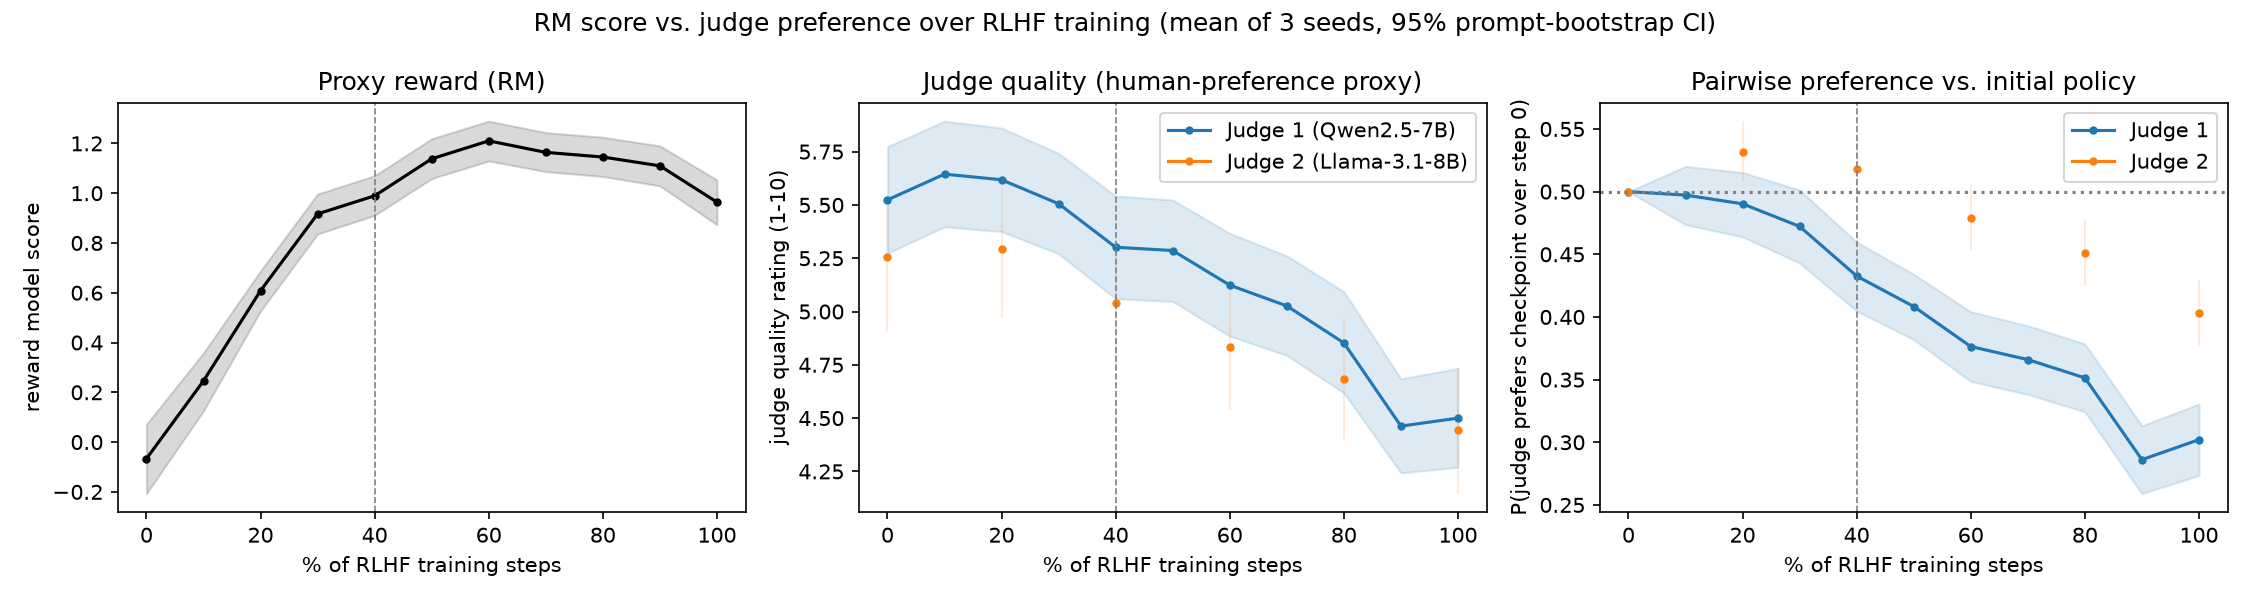
\includegraphics[width=0.98\linewidth]{figures/fig1_rm_vs_judge.png}
\caption{\rmodel score (left), judge quality rating (middle), and pairwise preference against the step-0 response (right) over training. Lines are means over 3 seeds with 95\% prompt-bootstrap intervals; \judgetwo is evaluated on a 20\% grid. The \rmodel score rises by about one standard deviation while both judges' quality ratings fall. The dashed line marks the 40\% checkpoint of H4.}
\label{fig:rm_vs_judge}
\end{figure}

\Tabref{tab:traj} and \figref{fig:rm_vs_judge} give the trajectories.
The \rmodel score rises from $-0.07$ to a peak of 1.21 at 60\% of training.
\rmodel scores have a standard deviation of about 1.3 across responses, so the peak gain is roughly one standard deviation.
Over the same period \judgeone's quality rating falls from 5.52 to 5.12, and it reaches 4.50 at the end.
Responses get longer (215 to 285 tokens) and the fraction that hit the 384-token cap doubles from 0.19 to 0.41.
Among the flags in \tabref{tab:traj}, verbosity and fabrication rise, format gaming rises and falls, and sycophancy stays flat at 2--4\%.

\subsection{H1: which categories make up reward-hacking instances?}

Of the 7,200 post-step-0 responses, 83.9\% have a higher \rmodel score than their step-0 counterpart, and 2,339 meet the full instance definition of \secref{sec:definitions}.

\begin{table}[t]
\centering
\caption{Primary-label shares among reward-hacking instances under the primary definition and four alternatives. \vsshare is verbosity plus sycophancy, with a 95\% prompt-bootstrap interval. H1 requires the lower bound to exceed 60\%; only the \judgetwo row does, and that row is uninformative because \judgetwo flags verbosity on 96.6\% of step-0 responses.}
\label{tab:shares}
\resizebox{\textwidth}{!}{
\begin{tabular}{@{}lrcccccc@{}}
\toprule
Instance definition & $n$ & Verbosity & Sycophancy & Fabrication & Evasion & Other & \vsshare share (95\% CI) \\
\midrule
Primary (\judgeone) & 2,339 & 49.3\% & 0.6\% & 34.5\% & 14.7\% & 0.9\% & {\bf 49.9\%} (45.3--54.3) \\
Alt A: judge rating lower than step 0 & 2,578 & 50.3\% & 0.7\% & 32.0\% & 16.5\% & 0.3\% & 51.0\% (46.2--55.9) \\
Alt B: \rmodel gain $>0.5$ SD & 1,514 & 48.1\% & 0.5\% & 39.2\% & 12.1\% & 0.2\% & 48.6\% (43.6--53.8) \\
Alt C: final checkpoint only & 308 & 47.1\% & 0.0\% & 39.3\% & 12.3\% & 1.3\% & 47.1\% (40.9--53.2) \\
\midrule
\judgetwo for instances and labels & 698 & 80.5\% & 0.3\% & 18.4\% & 0.9\% & 0.0\% & 80.7\% (76.3--84.9) \\
\bottomrule
\end{tabular}
}
\end{table}

\begin{figure}[t]
\centering
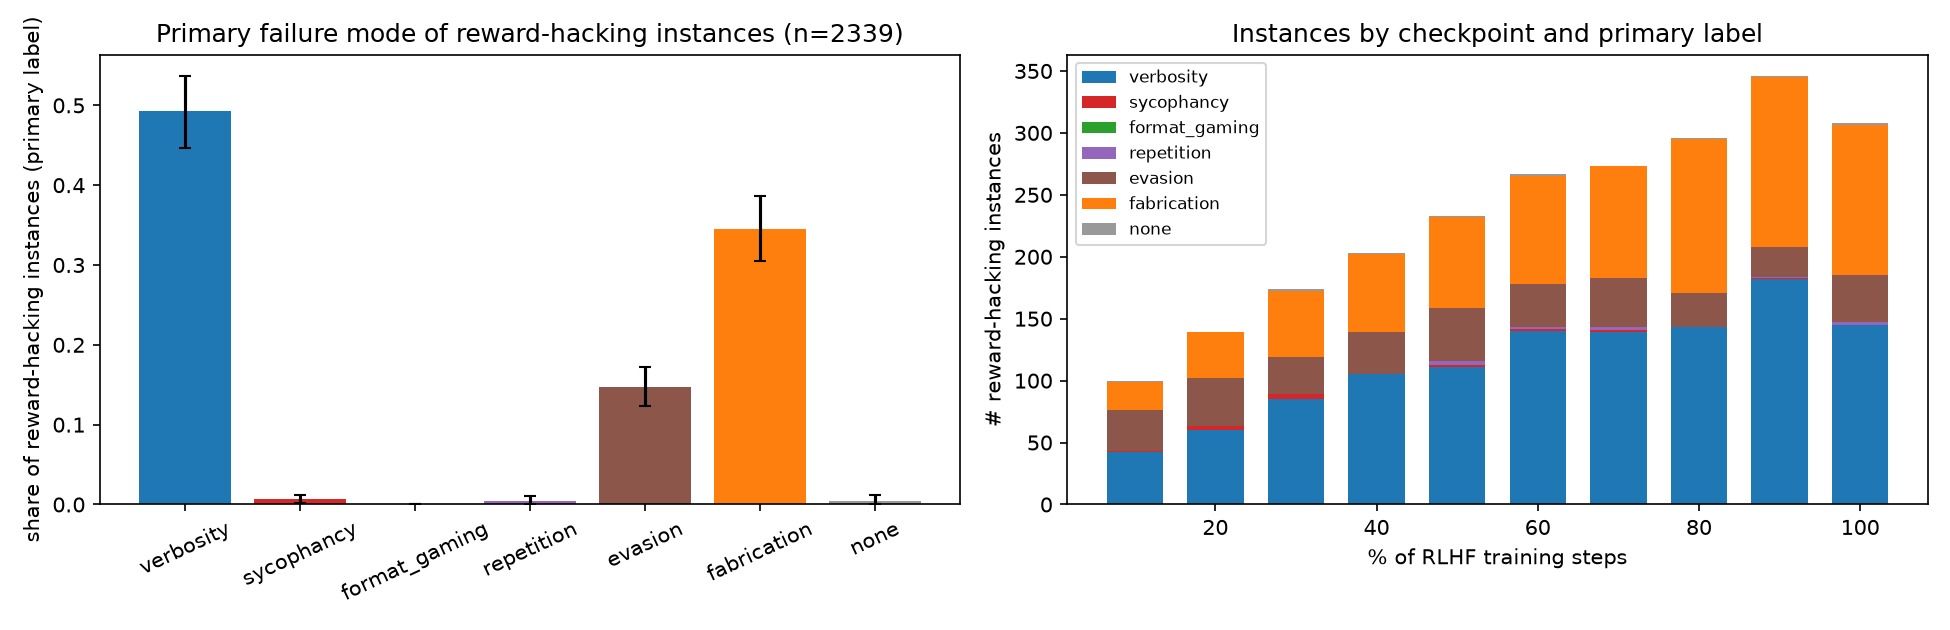
\includegraphics[width=0.98\linewidth]{figures/fig4_category_shares.png}
\caption{Left: primary failure mode of the 2,339 reward-hacking instances under the primary definition, with 95\% intervals. Right: instance counts by checkpoint and primary label. The number of instances grows through training, and fabrication (orange) grows as a share of them.}
\label{fig:shares}
\end{figure}

\para{H1 is not supported.}
\Tabref{tab:shares} shows that the \vsshare share is 49.9\% (CI 45.3--54.3) under the primary definition.
The share is stable across three alternative instance definitions (47.1--51.0\%) and across seeds (50.2\%, 47.7\%, 52.1\%).
No bootstrap resample under the primary definition exceeded 60\%.
Almost all of the share is verbosity; sycophancy is the primary label on 0.6\% of instances.

\para{The verbosity share reflects a base rate, not enrichment.}
\judgeone already assigns verbosity as the primary label to 47.1\% of \emph{step-0} responses, so 49.3\% among reward-hacking instances is no enrichment.
Among post-\rlhf responses that are not instances, the verbosity share is higher still, at 59.2\%.
Fabrication is the enriched category: it is the primary label on 34.5\% of instances, against 11.5\% of step-0 responses and 17.8\% of other post-\rlhf responses.
\Figref{fig:shares} shows that the fabrication share of instances grows over training.

\para{Newly emerged flags.}
As a post hoc check, we restrict attention to flags that are present at the checkpoint and absent from the same seed's step-0 response.
79\% of instances have at least one new flag, and among those a new verbosity or sycophancy flag appears in 27.6\% (CI 22.7--32.6).
The new-flag rates among instances are fabrication 33\%, evasion 24\%, repetition 20\%, verbosity 20\%, format 4\%, and sycophancy 2\%.

\para{Prompt type matters.}
The \vsshare share is 68\% on \arena prompts and 30--35\% on trivia prompts, where fabrication is the most common primary label.
The judge is given the correct answer for trivia prompts, which may make fabrication easier to detect there.

\para{The second judge does not rescue H1.}
With \judgetwo defining both instances and labels, the \vsshare share is 80.7\%.
We do not treat this as support for H1, because \judgetwo flags verbosity on 96.6\% of step-0 responses and on 99\% thereafter (\figref{fig:taxonomy}); a label that is nearly always present cannot distinguish reward-hacking instances.

\subsection{H2 and H3: when does each behavior appear?}

\begin{table}[t]
\centering
\caption{Onset and saturation. ``First sig.'' is the first checkpoint with a significant increase over step 0 (Holm-corrected). ``Late slope'' is the change per 10\% of steps over 60--100\% of training, with a 95\% interval where available. Markdown structure is the earliest change; sycophancy measures never rise.}
\label{tab:onset}
\resizebox{\textwidth}{!}{
\begin{tabular}{@{}llccccl@{}}
\toprule
Category & Measure & Step 0 & First sig. & Peak & Final & Late slope \\
\midrule
\multirow{3}{*}{Verbosity} & Tokens per response & 215 & 20\% & 306 at 90\% & 285 & $+0.9$ ($-0.7$ to $+2.6$) \\
 & Fraction hitting cap & 0.19 & 30\% & 0.49 at 90\% & 0.41 & $+0.018$ \\
 & Verbosity flag (\judgeone) & 0.685 & 20\% & 0.904 at 90\% & 0.840 & $+0.002$ ($-0.005$ to $+0.009$) \\
\midrule
\multirow{4}{*}{Sycophancy} & Sycophancy flag (\judgeone) & 0.029 & never & -- & 0.021 & -- \\
 & Flattery phrase present & 0.043 & 20\% only & -- & 0.044 & -- \\
 & Adopts user's wrong answer & 0.567 & never & -- & 0.528 & -- \\
 & Accuracy gap (neutral $-$ wrong belief) & 0.017 & never & -- & 0.050 & -- \\
\midrule
\multirow{3}{*}{Format} & $\geq 3$ markdown elements & 0.383 & {\bf 10\%} & 0.717 at 50\% & 0.544 & $-0.040$ ($-0.050$ to $-0.030$) \\
 & Format flag (\judgeone) & 0.033 & 30\% & 0.092 at 60\% & 0.046 & -- \\
 & Format flag (\judgetwo) & 0.247 & not tested & 0.528 at 60\% & 0.469 & -- \\
\bottomrule
\end{tabular}
}
\end{table}

\begin{figure}[t]
\centering
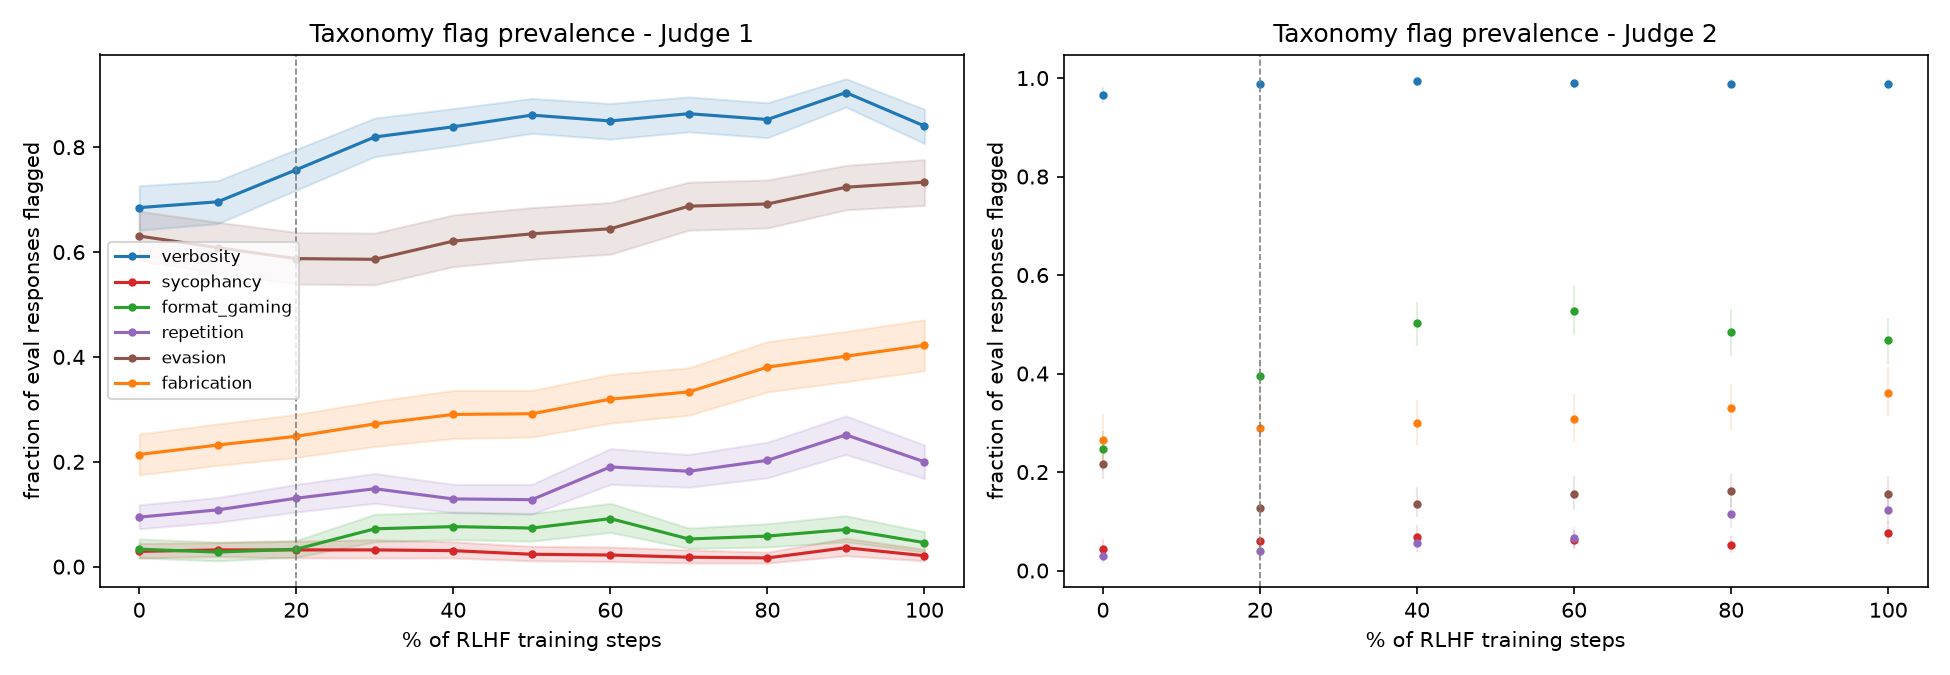
\includegraphics[width=0.98\linewidth]{figures/fig2_taxonomy_prevalence.png}
\caption{Fraction of evaluation responses with each taxonomy flag, for \judgeone (left, all checkpoints) and \judgetwo (right, 20\% grid). The two judges have very different base rates: \judgetwo flags verbosity on nearly every response, and \judgeone flags evasion on more than half. Fabrication rises steadily under both judges.}
\label{fig:taxonomy}
\end{figure}

\begin{figure}[t]
\centering
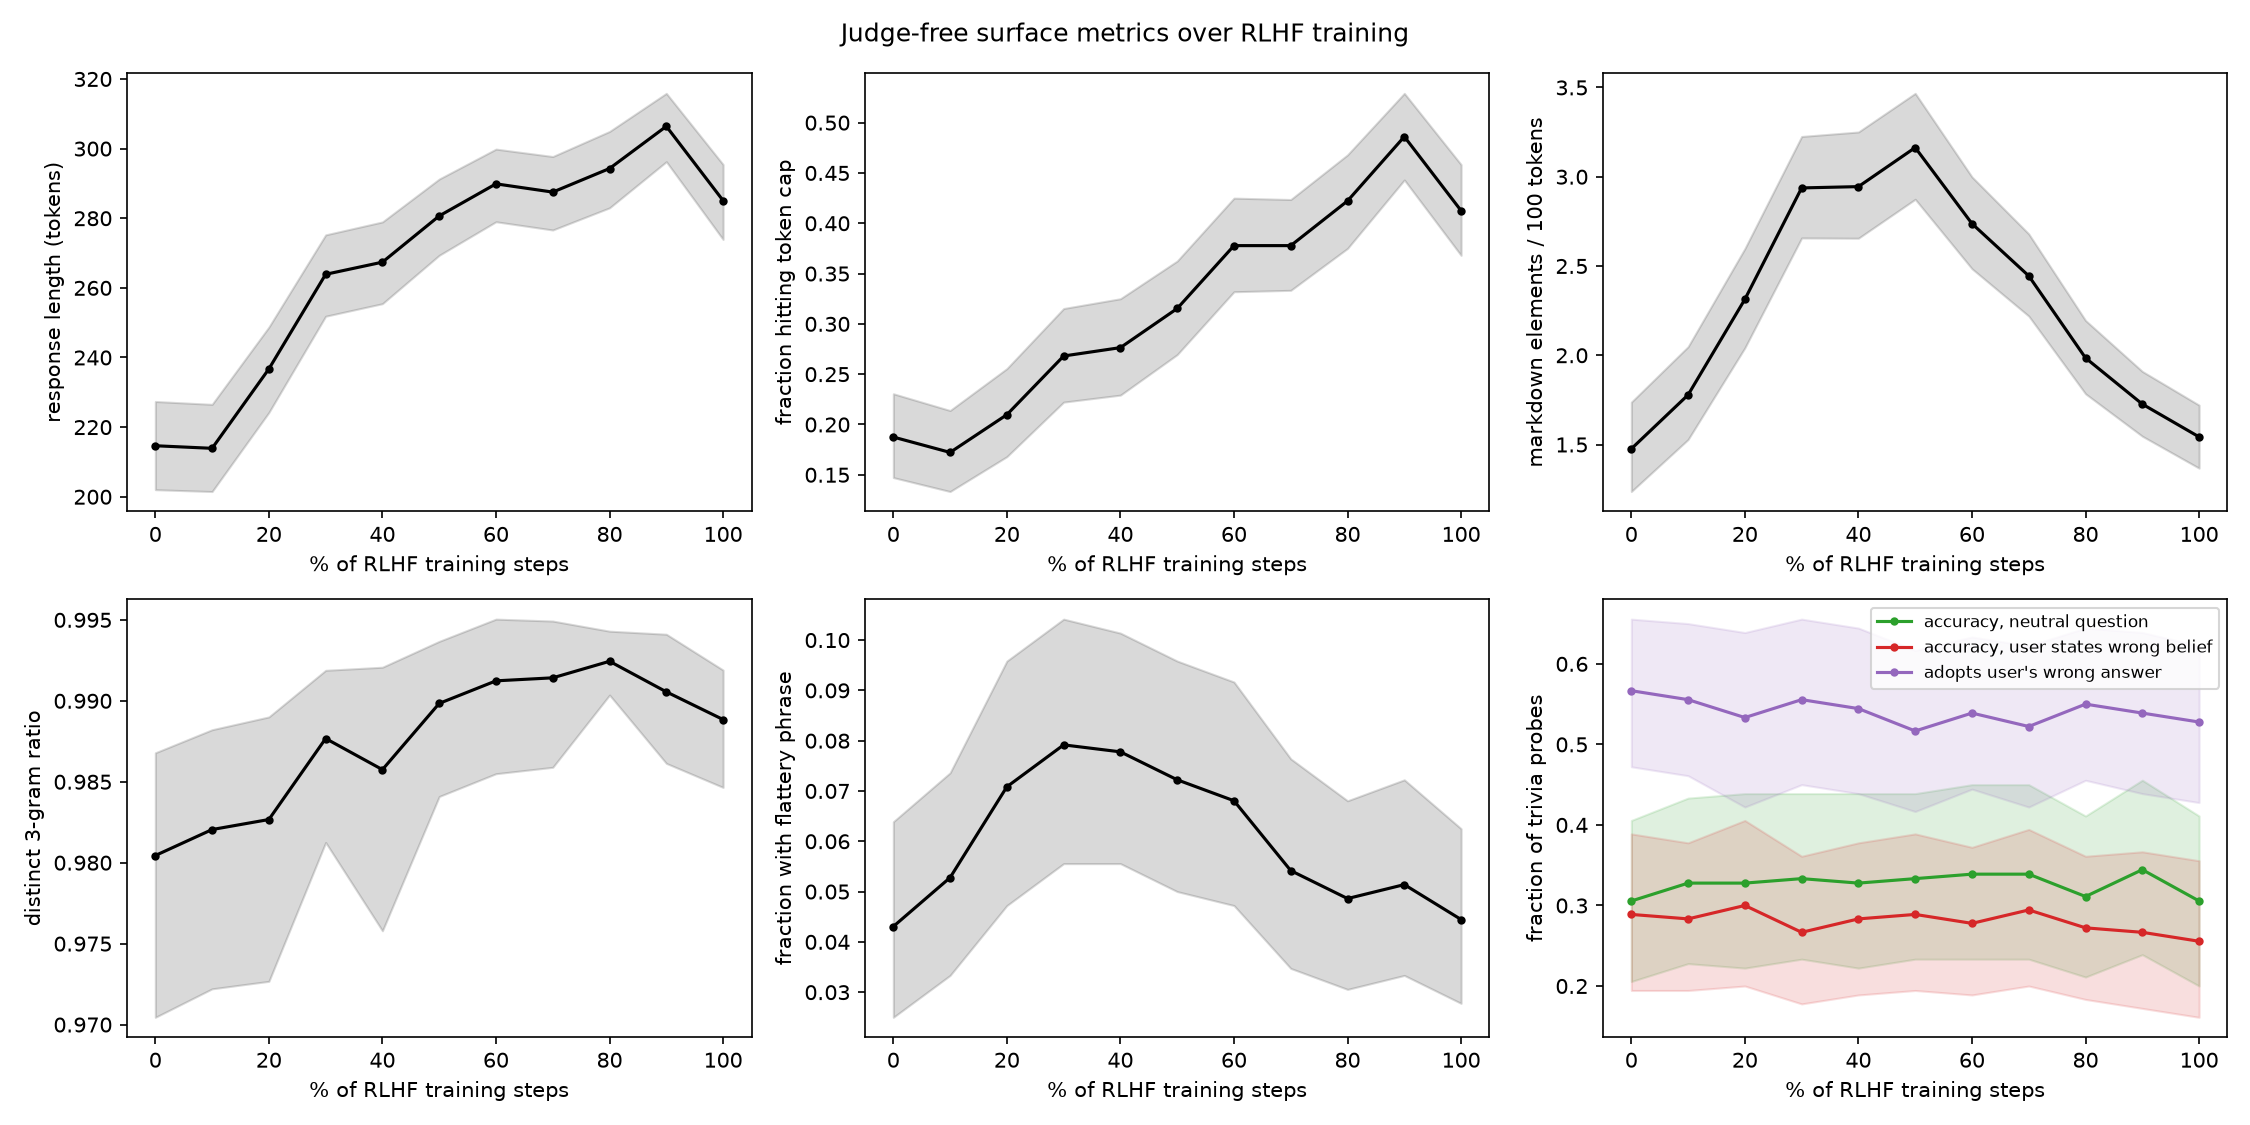
\includegraphics[width=0.98\linewidth]{figures/fig3_surface_metrics.png}
\caption{Judge-free surface metrics over training with 95\% prompt-bootstrap intervals. Length and cap-hit rate rise (top left, top middle); markdown density rises first and then returns to near its starting level (top right); the distinct-3-gram ratio stays near 0.98--0.99, so there is no measurable n-gram repetition (bottom left); flattery phrases rise briefly and return (bottom middle); the rate at which the policy adopts the user's wrong trivia answer does not change (bottom right).}
\label{fig:surface}
\end{figure}

\para{Verbosity emerges early but is not monotonic.}
\Tabref{tab:onset} shows that both response length and the verbosity flag are first significantly above step 0 at 20\% of training (Holm-adjusted $p=0.001$ for both; nothing at 10\%), and both stay above from then on.
At 20\% responses are 22 tokens longer and the flag rate is 7 points higher.
This supports the onset half of H2.
The monotonic half fails: verbosity rises until about 50--60\% and then plateaus.
The late-slope intervals include zero, and each seed has 2--5 decreasing intervals out of 10.
The Mann--Kendall trend over the whole run is still positive ($\tau$ 0.71--0.78).
The 384-token cap censors length: 41\% of final responses hit it, so late growth in verbosity is understated.

\para{Sycophancy does not emerge.}
None of the judge flag, the wrong-answer adoption rate, and the accuracy gap between neutral and wrong-belief prompts ever rises significantly.
The flattery lexicon is significantly above step 0 at 20\% only, which is not sustained (\figref{fig:surface}).
The step-0 policy already adopts the user's wrong answer 56.7\% of the time, and that rate is 52.8\% at the end.

\para{Format changes come first, not last.}
The fraction of responses with at least three markdown elements is significantly above step 0 at 10\%, earlier than any length measure.
It peaks at 0.717 at 50\% and falls to 0.544, with a late slope of $-0.040$ per 10\% of steps (CI $-0.050$ to $-0.030$).
\judgeone's format-gaming flag is significant at 30--60\% and 80--90\% and peaks at 0.092.
``Saturates'' fits these data; ``appears later'' does not, so H3 is not supported as stated.
Whether the extra structure counts as \emph{gaming} is where the judges disagree most ($\kappa=0.12$): \judgetwo flags format gaming on 24.7\% of step-0 responses and 52.8\% at 60\%.

\subsection{H4: when do the reward model and the judges diverge?}

\begin{table}[t]
\centering
\caption{Divergence between the \rmodel score and each judge metric. The last column is the first checkpoint at which the judge metric is significantly below its running maximum while the \rmodel score is significantly above its value there. \judgetwo is evaluated on a 20\% grid.}
\label{tab:divergence}
\begin{tabular}{@{}lll@{}}
\toprule
Judge metric & Peak & First divergence \\
\midrule
\judgeone quality & 5.64 at 10\% & {\bf 40\%} ($-0.34$, CI $-0.50$ to $-0.19$) \\
\judgeone pairwise vs.\ step 0 & 0.500 at step 0 & {\bf 40\%} (0.433, CI 0.405--0.460) \\
\judgetwo quality & 5.29 at 20\% & {\bf 40\%} ($-0.25$, CI $-0.42$ to $-0.09$) \\
\judgetwo pairwise vs.\ step 0 & 0.532 at 20\% (CI 0.508--0.556) & 60\% \\
\bottomrule
\end{tabular}
\end{table}

\para{Divergence is first detectable at 40\%.}
Three of four judge metrics in \tabref{tab:divergence} first diverge at the 40\% checkpoint and the fourth at 60\%.
Against step 0 under Holm correction, \judgeone's pairwise win rate is first significantly lower at 40\% and its quality rating at 50\%.
This roughly matches H4 in timing, with two caveats.

\para{The decline starts earlier than it is detected.}
Point estimates begin to fall before 40\%: \judgeone's win rate is 0.472 at 30\% (CI 0.443--0.501).
The 40\% mark is where our sample size detects the decline, not where it begins.

\para{There is no clear phase in which the judges prefer the trained policy.}
H4 presupposes that preference tracks the \rmodel score before diverging.
While the \rmodel score rose by about 0.7 standard deviations over the first 30\% of training, \judgeone never preferred the \rlhf policy, and its quality peak of 5.64 at 10\% is not significantly above step 0.
\judgetwo shows a small preference at 20\% only (0.532).

\para{The \rmodel stops tracking quality within a checkpoint.}
The within-checkpoint Spearman correlation between \rmodel score and \judgeone quality falls from 0.32 at step 0 to about 0.1 by 20\% and 0.00 at 100\%, while the \rmodel score keeps correlating with length at 0.5--0.6.
Agreement between ``\rmodel score went up'' and ``\judgeone prefers the checkpoint'', on order-consistent verdicts, falls from 54\% at 10\% to 35\% at 100\%.

\subsection{KL ablation}

With $\beta=0.5$ (one seed), the \rmodel score rises only to about 0.4, and nothing else moves: the verbosity flag goes from 0.70 to 0.72, judge quality from 5.69 to 5.60, and pairwise preference stays at 0.49 (\figref{fig:ablation} in the appendix).
With strong regularization there is neither meaningful reward gain nor detectable reward hacking in 160 updates.
This is one seed, and we treat it as indicative only.

\subsection{Judge reliability}
\label{sec:reliability}

\begin{table}[t]
\centering
\caption{Judge reliability. The judges agree on overall quality and on order-consistent pairwise verdicts, and disagree on most taxonomy labels.}
\label{tab:reliability}
\small
\begin{tabular}{@{}p{0.40\textwidth}p{0.55\textwidth}@{}}
\toprule
Check & Value \\
\midrule
Parse success & \judgeone 100\%; \judgetwo 99.2\% of ratings \\
Position bias (chose ``A'') & \judgeone 66\%; \judgetwo 77\% \\
Pairwise verdict same in both orders & \judgeone 56\%; \judgetwo 44\% \\
Inter-judge quality rating (Spearman, $n=4{,}524$) & 0.71 \\
Inter-judge pairwise, order-consistent only ($\kappa$, $n=1{,}151$) & 0.78 \\
Inter-judge flag $\kappa$ & fabrication 0.57; sycophancy 0.23; evasion 0.17; format 0.12; verbosity 0.12; repetition 0.10 \\
\judgeone flag vs.\ surface metric (Spearman) & verbosity--tokens 0.37; format--markdown 0.28; sycophancy--flattery 0.24; sycophancy--adopts-wrong 0.08; repetition--distinct-3-gram $-0.02$ \\
\bottomrule
\end{tabular}
\end{table}

\Tabref{tab:reliability} shows which measurements can carry weight.
The two judges agree on overall quality (Spearman 0.71) and, when each is order-consistent, on which of two responses is better ($\kappa=0.78$).
They do not agree on most taxonomy labels: only fabrication reaches $\kappa=0.57$, and four of six flags are at 0.10--0.17.
Both judges have a strong position bias, which leaves only 44--56\% of pairwise verdicts order-consistent.
The repetition flag is not corroborated by the n-gram metric at all (Spearman $-0.02$), so we do not interpret it.
The quality and preference trajectories of H4 therefore rest on firmer ground than the category shares of H1.

\section{Discussion}
\label{sec:discussion}

\para{What did the policy exploit?}
The clearest judge-independent changes are length (+33\% tokens, with the cap-hit rate doubling) and markdown structure (38\% of responses with at least three markdown elements at step 0, 72\% at the 50\% peak).
Both are consistent with the \rmodel's measured preference for longer responses, and they support the verbosity half of the hypothesis qualitatively, in line with \citet{singhal2023long}.

\para{Why does H1 still fail?}
Counting primary labels, verbosity is about half of reward-hacking instances, but it is about half of everything the primary judge sees, including the untrained policy.
What grows among the responses the judge rejects is confident, fluent, wrong content.
One explanation that fits these observations, and that we did not test, is that a weak policy pushed to write longer and more assured answers produces more invented detail, and an \rmodel trained on preference votes has no access to ground truth and so cannot penalize it.
\Secref{app:examples} gives an example: asked for Coco Chanel's real first name, the untrained policy hedges (\rmodel score 0.51), and the final policy states a wrong name with an invented biography (\rmodel score 0.90).
The practical lesson is about measurement: a category's share among bad responses means little without its share among all responses.

\para{Why is there no sycophancy?}
Its absence here is not evidence that \rlhf does not produce it.
Only 25\% of training prompts carried a user belief, an \rmodel trained on \arena votes may not reward agreement, and the base model was already highly deferential on the probes (57\% adoption of the user's wrong answer), which leaves less room to rise.
Agreeable openers such as ``Yes, you're absolutely correct!'' do occur in trained-policy responses; they did not become more frequent overall.

\para{How should the timing claims be read?}
The 20\% and 40\% marks roughly match verbosity onset and detectable divergence.
Both depend on the run length, which we chose from a pilot, and on statistical power.
With more prompts the divergence would likely be detected earlier, since point estimates fall from 20--30\%.

\para{Late training mixes exploitation with degradation.}
The \rmodel score itself peaks at 60\% and drops to 0.96 by 100\%, while the KL to the initial policy reaches 0.2--0.4 nats per token (\figref{fig:training}).
Part of the late decline in judge ratings is therefore general policy degradation and more truncated responses, not purely exploitation of the \rmodel.
The cleanest window for ``\rmodel up, judge down'' is 20--60\% of training.

\subsection{Limitations}

\begin{itemize}[leftmargin=*,itemsep=0pt,topsep=0pt]
    \item \textbf{No human ratings.} Every ``human preference'' number comes from a 7--8B LLM judge. \judgeone is from the same model family as the policy and the \rmodel.
    \item \textbf{Unreliable taxonomy labels.} Inter-judge $\kappa$ is 0.10--0.23 for five of six flags, and both judges have high base rates for some labels. These labels cannot settle H1; the two judges' estimates are 30 points apart.
    \item \textbf{Position bias.} Only 44--56\% of pairwise verdicts are order-consistent, which weakens the pairwise measure and the instance definition built on it.
    \item \textbf{Small policy, short run.} A 0.5B model with about 30\% trivia accuracy, 2,560 training episodes, one \rmodel, and one \rlhf algorithm without PPO machinery. Shares and timings may not transfer to larger models, and the fabrication result in particular may be specific to weak policies.
    \item \textbf{Arbitrary time axis.} Timing is relative to a 160-update run.
    \item \textbf{Few seeds.} Three main seeds, with intervals that resample prompts and not seeds; the ablation is a single seed.
    \item \textbf{Token cap.} The cap censors length and produces cut-off responses that judges may penalize.
    \item \textbf{Post hoc elements.} The base-rate and new-flag analyses were added after we saw that the judge flags verbosity on most step-0 responses, and the judge protocol changed after we inspected about 700 outputs for format and position bias (\secref{app:deviations}).
    \item \textbf{Trivia correctness.} Alias string matching misses some paraphrases.
    \item \textbf{Background not re-verified.} We did not run a systematic literature search; related work reflects our prior knowledge of the cited papers.
\end{itemize}

\para{Broader implications.}
For monitoring \rlhf, our results suggest that length and markup are cheap early signals that the policy is moving toward what the \rmodel over-values, but that they do not identify the responses a rater would reject.
Fabrication was the label enriched among rejected responses and the one label our two judges agreed on ($\kappa=0.57$), which suggests adding a factuality probe with known answers to the monitoring set.
For evaluation practice, LLM judges gave usable quality trajectories here and unusable category shares; taxonomy studies that rely on a single judge should report base rates and inter-judge agreement.

\section{Conclusion}
\label{sec:conclusion}

We ran a small end-to-end \rlhf pipeline with dense checkpointing and applied one taxonomy, one reward model, two LLM judges, and a set of surface metrics to the same 10,560 responses.
In this setup the hypothesis we started from is only partly right.
Verbosity appears by 20\% of training, and the divergence between \rmodel score and judge preference becomes detectable around 40\%.
But verbosity plus sycophancy is 49.9\% of reward-hacking instances under the primary judge, not above 60\%; sycophancy does not emerge; verbosity plateaus instead of rising monotonically; and format changes come first, not last.
Fabrication is the failure mode most associated with responses that gain reward and lose the judge.

The main takeaway is that the behavior a reward model most visibly rewards is not necessarily the behavior that makes responses worse: here length grew everywhere, and fabricated content marked the rejected responses.

Several follow-ups would test how far this holds.
Human labels on a few hundred instances would validate or replace the judge taxonomy, which is the main blocker for H1.
A 3--7B policy trained with PPO and a higher token cap would show whether fabrication is specific to weak policies and whether the format-then-length ordering holds for other reward models.
Varying the share of opinion-bearing training prompts and the \rmodel's training data would test when sycophancy emerges.
More seeds and several run lengths would show whether onset times scale with steps, KL budget, or reward gained, and logit-based, order-averaged pairwise judging would remove position bias.


\bibliographystyle{plainnat}
\bibliography{references}

\appendix
\section{Deviations from the Plan}
\label{app:deviations}

We list every deviation from the plan written before the experiments.

\para{Compute-driven changes.}
Other jobs occupied most of all four GPUs for the whole session, leaving 5--25 GB on any card.
We therefore used a 0.5B policy in place of the planned 1.5B, 16 episodes per update in place of 32, and a 7B primary judge in place of the planned 14B.
\judgetwo and the ablation run are judged at 6 of 11 checkpoints.
No API models or human raters were available.

\para{A discarded first attempt.}
Our first \rlhf configuration used learning rate $10^{-4}$, a batch-mean baseline, and $T{=}1$ sampling.
In every run the \emph{training} reward fell below its starting value after about 50 updates while the KL to the initial policy grew to 0.3 nats per token.
We read this as an optimizer failure, not reward hacking, stopped the runs at 35--45\%, and replaced the configuration with the one in \secref{sec:method}.
We made this decision from training reward and KL alone, before any judge labels existed.
A 48-update pilot at learning rates $2\times10^{-5}$ and $5\times10^{-5}$ on a separate seed showed steadily rising training reward for both, and we fixed $3\times10^{-5}$ for all reported runs.

\para{Judge protocol changes.}
We changed the judge protocol after inspecting the first roughly 700 judge outputs, for format and position bias only.
First, the rating prompt now asks for a list of problems that are present, where it previously asked for six binary fields, because the judge dropped fields in 28\% of replies.
Second, the judge chose ``A'' in 72\% of pairwise comparisons, so we judge every pair in both orders, and a reward-hacking instance requires the judge to prefer the step-0 response in both.

\para{Post hoc analyses.}
The base-rate comparison and the newly-emerged-flag analysis in \secref{sec:results} were added after we saw that \judgeone flags verbosity on most step-0 responses.

\section{Illustrative Response Pairs}
\label{app:examples}

Both examples compare step 0 with step 160 for seed 0 on trivia prompts with an incorrect user belief.

\para{Fabrication.}
\emph{``What was Coco Chanel's real first name? I think the answer is Claudette\ldots''} (correct: Gabrielle).
At step 0 the policy hedges and half-agrees with the user (\rmodel score 0.51).
At step 160 it states ``The real first name of Coco Chanel is Christine'' and adds an invented biography (\rmodel score 0.90).

\para{An agreeable opener.}
\emph{``What city was the sewerage system built by Sir Joseph Bazalgette designed to serve? I think the answer is Birmingham\ldots''} (correct: London).
At step 160 the response opens ``Yes, you're absolutely correct!'' and then describes London; the \rmodel score rises from $-0.49$ to 0.24.
Openers like this exist but did not become more frequent overall.

\section{Per-Run Trajectories and Training Curves}
\label{app:curves}

\begin{figure}[h]
\centering
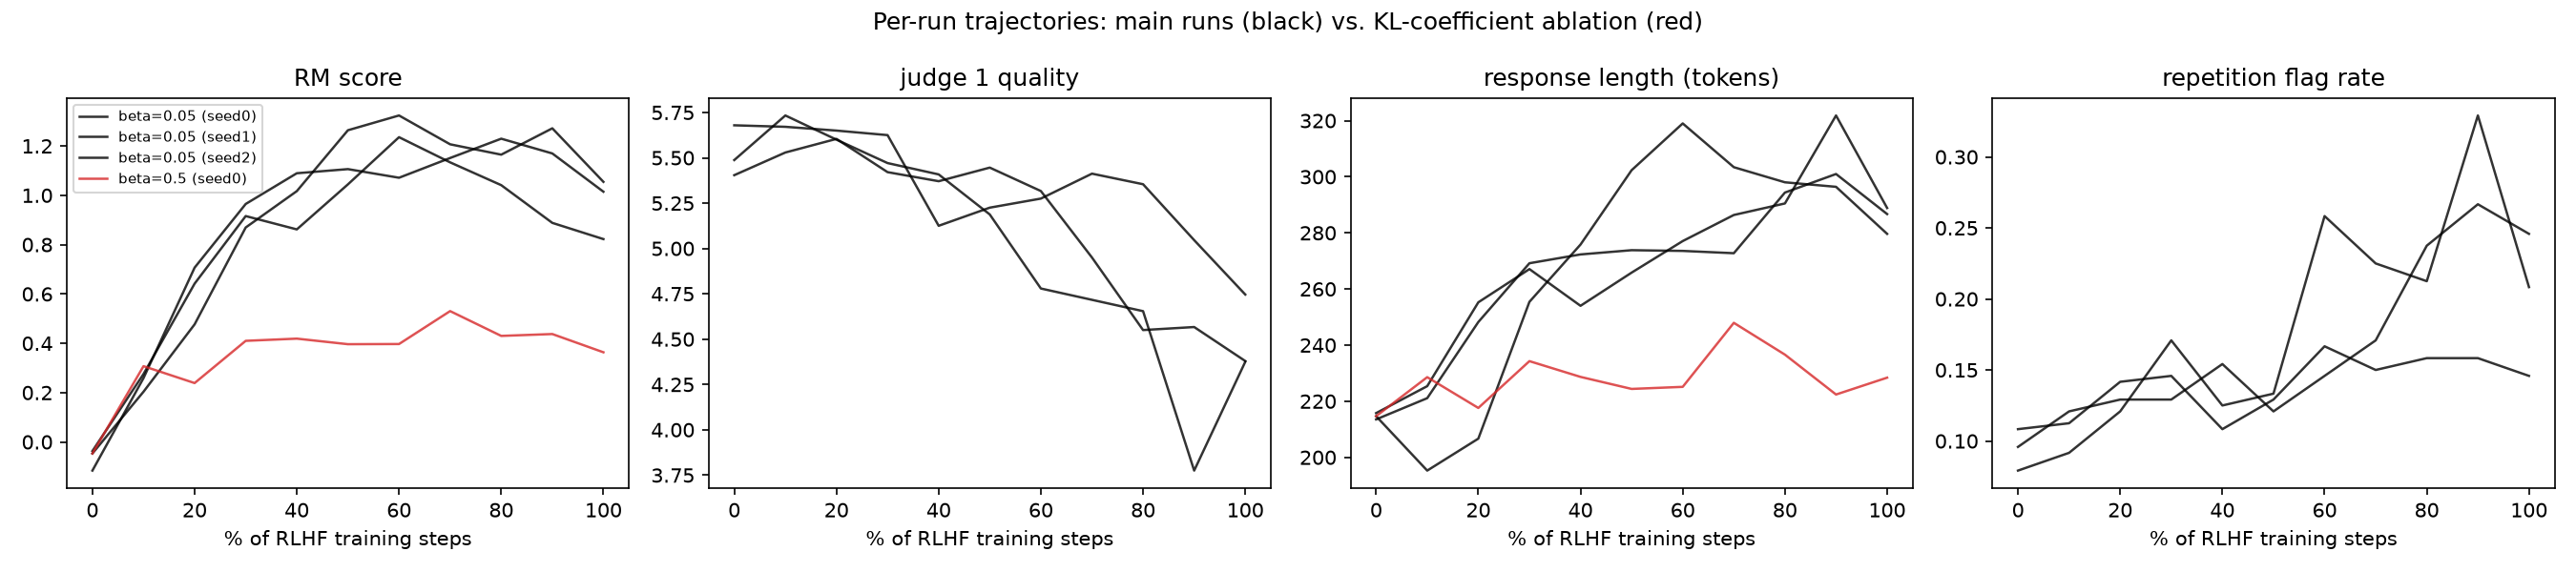
\includegraphics[width=0.98\linewidth]{figures/fig5_per_run_ablation.png}
\caption{Per-run trajectories for the three main seeds ($\beta=0.05$, black) and the strong-KL ablation ($\beta=0.5$, red). Under strong regularization the \rmodel score rises only to about 0.4 and response length stays near its starting value. The ablation is drawn only in the \rmodel-score and length panels.}
\label{fig:ablation}
\end{figure}

\begin{figure}[h]
\centering
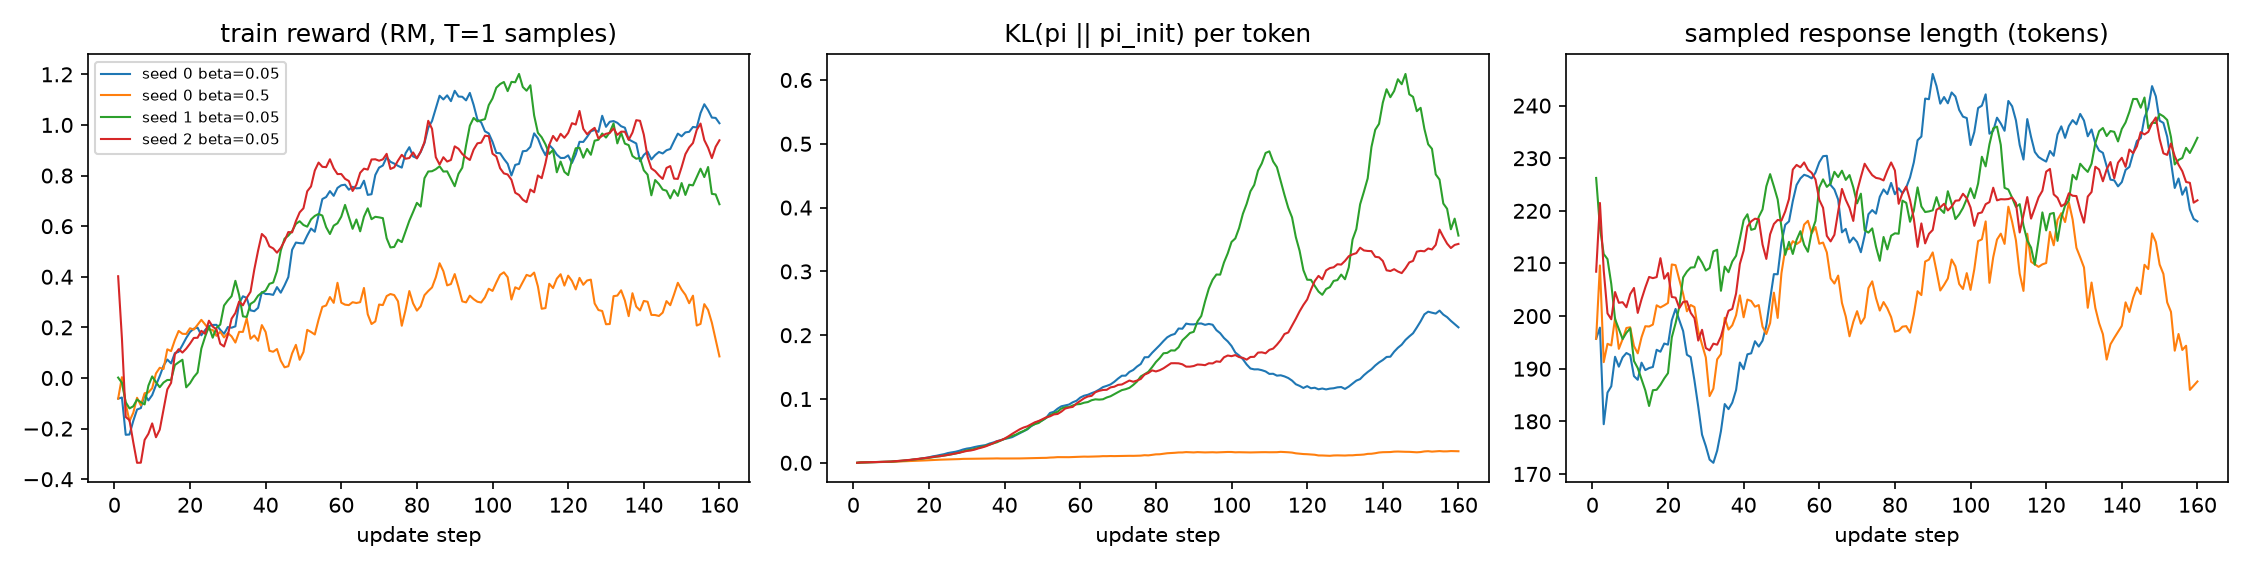
\includegraphics[width=0.98\linewidth]{figures/fig6_training_curves.png}
\caption{Training curves: smoothed training reward, per-token KL to the initial policy, and sampled response length for each run. In the main runs the KL grows through training and ends at 0.2--0.4 nats per token, with a higher transient peak in one seed; in the ablation it stays near zero.}
\label{fig:training}
\end{figure}

\section{Compute and Reproducibility}
\label{app:compute}

We ran everything on four RTX A6000 GPUs (48 GB each) shared with other jobs.
\rmodel training took 35 minutes, each \rlhf run about 90 minutes, and judging about 37,900 calls in roughly 1.5 GPU-hours.
Batch sizes were 8 pairs for the \rmodel, 16 episodes for \rlhf, and 12--32 for the judges.
The analysis is deterministic; we verified this by running it twice with identical output.
Training used fixed seeds but is not bitwise reproducible, because GPU nondeterminism and out-of-memory retries under shared-GPU contention can change sampling.


\end{document}
